\documentclass[amtd, online, hvmath]{copernicus}

\begin{document}\hack{\sloppy}

\title{The Aerosol Limb Imager: acousto-optic imaging of limb scattered
sunlight for stratospheric aerosol profiling}

\Author{B.~J.}{Elash}
\Author{A.~E.}{Bourassa}
\Author{P.~R.}{Loewen}
\Author{N.~D.}{Lloyd}
\Author{D.~A.}{Degenstein}

\affil{Institute of Space and Atmospheric Studies, Saskatchewan,
Canada}


\correspondence{B.~J.~Elash (brenden.elash@usask.ca)}

\runningtitle{The Aerosol Limb Imager}
\runningauthor{B.~J.~Elash et~al.}


\received{26~October~2015}
\accepted{30~November~2015}
\published{}


\firstpage{1}

\maketitle


\begin{abstract}
  The Aerosol Limb Imager (ALI) is an optical remote sensing
  instrument designed to image scattered sunlight from the atmospheric
  limb. These measurements are used to retrieve spatially resolved
  information of the stratospheric aerosol distribution, including
  spectral extinction coefficient and particle size. Here we present
  the design, development and test results of an ALI prototype
  instrument. The long term goal of this work is the eventual
  realization of ALI on a~satellite platform in low earth orbit, where
  it can provide high spatial resolution observations, both in the
  vertical and cross-track. The instrument design uses a~large
  aperture Acousto-Optic Tunable Filter (AOTF) to image the sunlit
  stratospheric limb in a~selectable narrow wavelength band ranging
  from the visible to the near infrared. The ALI prototype was tested
  on a~stratospheric balloon flight from the Canadian Space Agency
  (CSA) launch facility in Timmins, Canada, in
  September~2014. Preliminary analysis of the hyperspectral images
  indicates that the radiance measurements are of high quality, and we
  have used these to retrieve vertical profiles of stratospheric
  aerosol extinction coefficient from 650--1000\,\unit{nm}, along with
  one moment of the particle size distribution. Those preliminary
  results are promising and development of a~satellite prototype of
  ALI within the Canadian Space Agency is ongoing.
\end{abstract}


\introduction

Stratospheric aerosol plays an important role in the global radiative
forcing balance by scattering solar irradiation and causing an overall
cooling effect that depends on the particle size distribution and the
concentration (Kiehl and Briegleb, 1993; Stocker et~al., 2013). These
climate effects are an important and recent focus of research due to
the potential contribution of stratospheric aerosol to the so-called
global warming hiatus (Solomon et~al., 2011; Haywood et~al., 2014;
Fyfe et~al., 2013), and efforts to quantify the variability and trends
in the global stratospheric aerosol load are underway with various
ground based and satellite data sets (Rieger et~al., 2015; Ridley
et~al., 2014).

Since its discovery with stratospheric balloon observations (Junge
et~al., 1961), stratospheric aerosol has been measured with various
techniques, although due to the variability of physical composition
and particle size, no single measurement technique can determine the full range of aerosol properties unambiguously. In-situ balloon observations continue to be used and have
provided highly valuable data sets, including most notably the long
time series of optical particle counter measurements from Laramie, WY
(Deshler et~al., 2003, 2006; Kovilakam et~al., 2015). Aircraft-borne
nephelometers (Beuttell and Brewer, 1949; Charlson et~al., 1969)
acquire detailed in-situ measurements, providing, for example, plume
composition (Murphy et~al., 2014), but are spatially limited to the
aircraft track. Ground based lidars have been used to do detailed
studies of the extent of volcanic aerosol plumes (Chazette et~al.,
1995; Sawamura et~al., 2012) and provide valuable insight into long
term local variability and trends in the aerosol layer. For example,
lidar observations were used by Hofmann et~al.~(2009) to first report
the observed increase in stratospheric aerosol over approximately the
last decade. However, the global distribution, which can only really
be obtained with satellite observations, provides invaluable insight
into aerosol processes and variability. A~good example of this is the
use of satellite observations by Vernier et~al.~(2011b) to determine
that the increased stratospheric aerosol load reported by Hofmann
et~al.~(2009) was in fact due to a~series of relatively minor, mostly
tropical, volcanic eruptions.

Satellite instrumentation capable of remote sensing stratospheric
aerosol has been in use since the 1970s, beginning with limb sounding
solar occultation measurements. These have provided a~reliable,
accurate and essentially continuous long term record of vertically
resolved aerosol extinction coefficient measurements, mostly from the
series of Stratospheric Aerosol and Gas Experiment (SAGE) instruments
(Russell and McCormick, 1989; Thomason and Taha, 2003). These SAGE
measurements, which have a~vertical resolution of approximately
1\,\unit{km}, have generally compared well with ground based and
in-situ measurements, although there are challenges associated with
determining microphysical
parameters and comparison between instruments can be challenging. (Russell and McCormick, 1989; Kovilakam et~al.,
2015). However, solar occultation is generally a~robust and stable
technique as it directly measures atmospheric optical depth, along
with the exo-atmospheric solar spectrum with each scan, allowing for
straightforward retrieval of aerosol extinction coefficient (Damadeo
et~al., 2013). The SAGE III mission came to an end in 2006 and the occultation measurements have continued from the currently operational MAESTRO and
ACE-Imager instruments on SciSat (McElroy et~al., 2007; Gilbert
et~al., 2007) and have had some success producing stratospheric aerosol
extinction products (Vanhellemont et~al., 2008; Sioris et~al., 2010).
Furthermore, a~manifestation of SAGE III is planned
for deployment on the International Space Station in 2016 (Cisewski
et~al., 2014).

More recently, limb scattered sunlight measurements have been used for
stratospheric aerosol retrievals. Although this technique has the
advantage of being able to sample the atmosphere throughout the sunlit
hemisphere, it requires the use of a~complex forward model of multiple
scattering processes along with at least some a~priori knowledge of
the aerosol scattering cross section in order to retrieve the
extinction coefficient profile. The Optical Spectrograph and InfraRed
Imaging System (OSIRIS) instrument (Llewellyn et~al., 2004), which was
launched in 2001 and is presently still operational, was the first
satellite limb scatter instrument to retrieve stratospheric aerosol
extinction (Bourassa et~al., 2007). The current OSIRIS version 5.07
data product, which provides 750\,\unit{nm} extinction profiles at
approximately 2\,\unit{km} vertical resolution, has been shown to
agree relatively well, generally below 30\% below 30\,\unit{km}, with SAGE II and SAGE III occultation
measurements  (Bourassa et~al., 2012b; Rieger et~al., 2015). The
SCanning Imaging Absorption spectroMeter for Atmospheric CHartographY
(SCIAMACHY) instrument on Envisat (Bovensmann et~al., 1999) uses
a~retrieval technique essentially similar to OSIRIS to retrieve
aerosol profiles at 750\,\unit{nm} with approximately 3\,\unit{km}
vertical resolution (Taha et al., 2011; Ernst et~al., 2012; von Savigny et~al., 2015)
from scattered sunlight spectra.  SCIAMACHY observations ceased with
the demise of Envisat in 2012 and although OSIRIS continues to
operate, it is now in the fourteenth year of a~mission designed for
two years.

The most recently launched limb scatter instrument is the Ozone
Mapping Profiler Suite Limb Profiler (OMPS-LP) on the Suomi-NPP
satellite. Although similar in spectral range and vertical resolution
to OSIRIS, OMPS-LP is an imaging spectrometer that vertically images
the limb in a~single measurement. Both OSIRIS and SCIAMACHY are
grating spectrometers with a~narrow field of view, such that limb
profiles are obtained by vertically scanning through a~range of
tangent altitudes. The imaging capability of OMPS provides a~decrease
in the time required to obtain a~limb profile and so increases the
along track sampling. Recent work on the feasibility of aerosol
retrieval from OMPS-LP measurements show promising results (Rault and
Loughman, 2013).

Several recent studies have highlighted the requirement for continued global
stratospheric aerosol observations, and especially the need to resolve, both
vertically and horizontally, aerosol in the lowermost stratosphere and the
upper troposphere. This is the case for tracking the evolution of aerosol
from volcanic eruptions, which can have a~substantial effect on the aerosol
optical depth in the lowermost stratosphere (Ridley et~al., 2014; Andersson
et~al., 2015). Furthering the understanding of the transport of aerosol near
and across the tropopause would also benefit from higher spatial and temporal
resolution observations. This is evident in the case of volcanic plumes, such
as that from Nabro in 2011, the transport and origin of which has been
studied extensively and the conclusions are somewhat controversial (Bourassa et~al., 2012c,
2013; Vernier et~al., 2013; Fromm et~al., 2013, 2014; Fairlie et~al., 2014;
Clarisse et~al., 2014). However, this is also the case for the formation of
background-level aerosol, particularly in the region of the Asian and North
American monsoons, which have been identified as a~source of substantial,
seasonal and highly structured aerosol formation from precursor, tropospheric
source gases (Vernier et~al., 2011a; Neely et~al., 2014; Thomason and
Vernier, 2013).

Many of the studies mentioned above have involved the use of Cloud
Aerosol Lidar and Infrared Pathfinder Satellite Observation (CALIPSO)
space-borne lidar measurements (Winker et~al., 2007), which nominally
measures backscatter profiles approximately every 300\,\unit{m} along
track with approximately 200\,\unit{m} vertical resolution. However,
the stratospheric backscatter signal is weak and requires averaging of
only the night time measurements over several days and typically
0.5\,\unit{km} vertically and 500\,\unit{km} horizontally (Vernier
et~al., 2011b). Additionally, the uncertainty in the calibration with
respect to the molecular background that is on the order of the
stratospheric aerosol signal leads to a~potential bias in the
stratospheric measurements (Rogers et~al., 2011). CALIPSO was launched
in 2006 and although it is presently still operational, it is also
operating beyond its design lifetime. More recently the lidar instrument Cloud Aerosol Transport System (CATS) (Chuang et al., 2013) has been placed on the international space station in 2015 for an expected mission lifetime of three years.

Continued stratospheric aerosol observations from space are
drastically needed though few, if any, planned missions with such
capability are underway. In this paper we present the design and test
of a~prototype instrument for potential future satellite-based
stratospheric aerosol observation. The Aerosol Limb Imager (ALI)
concept is a~relatively small, low-cost, low-power, passive
instrument, suitable for microsatellite deployment, with the
capability to provide high spatial resolution measurements, both
vertically and horizontally, of the visible/NIR aerosol extinction
coefficient. The basic idea is to leverage the clear advantages of the
limb scatter technique as a~passive, and therefore low mass and power,
means to obtain daily global coverage, with a~two dimensional
hyperspectral imager for filling cross-track observation.

The ALI instrument concept is built around the use of an Acousto-Optic
Tunable Filter (AOTF), which is a~novel filtering technology that
provides the ability to rapidly select the central wavelength of an
image with no moving parts. These filters, which have recently been
developed as large aperture, imaging quality devices, operate very
efficiently in the red and near infrared spectral range, which is
a~well matched spectral range for limb scatter sensitivity to aerosol
and cloud (Rieger et~al., 2014).  Additionally, the spectral bandpass
of the AOTF has reasonable resolutions at these
wavelengths such as 3--6\,\unit{nm}, which is very suitable for the broadband scattering
characteristics of the aerosol limb signal. The two dimensional
imaging nature of the design provides the capability to achieve at
least sub-kilometer resolution at the tangent point, which is on the
order of the scale size of the upper troposphere and lower
stratosphere (UTLS) aerosol features mentioned above.

It should be noted that the basic instrument design concept of ALI is
very similar to that of the Atmospheric Limb Tracker for the
Investigation of the Upcoming Stratosphere (ALTIUS) (Dekemper et~al.,
2012), which is a~Belgian instrument concept from the Belgian
Institute for Space Aeronomy (BIRA).  ALTIUS is designed to measure
limb scattered sunlight; however, it also has solar, stellar, and
planetary occultation modes and is scientifically focused on trace gas
measurements, particularly for ozone, whereas ALI is optimized for
aerosol observation.

\section{ALI instrument design}

ALI is a~simple optical system that images essentially a~single
wavelength at a~time through the use of an acousto-optic tunable
filter (AOTF). The AOTF is a~unique device that allows for the
filtering without any moving parts and relatively low power
consumption. However, the AOTF operation requires important instrument
design considerations to account for its optical operation. For
example, the diffractive qualities of the AOTF depend on the angle
that light enters the device. Additionally, in practice the AOTF
output is limited to a~single linear polarization, which reduces the
system throughput and causes potential internal stray light in the
system through the rejection of the other linear polarization. The
following sections provide a~brief introduction to the physical
operation of the AOTF, considerations for implementation in a~system
designed specifically for aerosol, and an overview of the final ALI
optical design.

\subsection{Acousto-optical tunable filter}

The primary filtering device behind ALI and the technology that allows
for the two dimensional spatial imaging is the AOTF, which is
typically made from a~birefringent crystal. A~radio frequency (RF)
wave is propagated through the crystal, and forms an acoustic shear
wave that interacts with an incoming beam of light in an effect
similar to the diffraction of a~specific wavelength. The use of an
AOTF for an imaging system has several distinct advantages due to its
low mass, fast stabilization times of a~few microseconds, and no
moving parts. Although many applications use small, non-imaging AOTFs
with various configurations, large aperture, birefringent,
non-collinear acousto-optic devices are typically used in imaging
systems. A~non-collinear device is one where the input light beam and
the RF acoustic wave are not aligned. Thanks to recent advancements in
non-collinear AOTF technology these devices now have relatively high
efficiency and robust imaging quality (Georgiev et~al., 2002;
Voloshinov et~al., 2007).

To create the diffraction of a~specific wavelength, a~momentum matching
criterion must be held where the wave vectors of the acoustic wave match the
difference of the incoming and diffracted light wave vectors as seen in
Fig.~1. This condition is known as the Bragg matching criterion and is given
by
\begin{align}
\vec{k}_{\mathrm{i}}=\boldsymbol{\kappa} +\vec{k}_{\mathrm{d}}
\end{align}
where $\left| \vec{k}_{\mathrm{i}} \right|\,=\,2\pi
n_{\mathrm{i}}/\lambda$ is the wave number of the incident light,
$\left| \vec{k}_{\mathrm{d}} \right|\,=\,2\pi n_{\mathrm{d}}/\lambda$
is the wave number of the diffracted light, and $\left|
  \boldsymbol{\kappa} \right|\,=\,2\pi F/\nu$ is the wave number of
the acoustic wave. The parameters $\lambda$, $F$ and $\nu$ are the
wavelength of light in vacuum, the frequency of the RF wave, and the
phase velocity in the crystal respectively and the indices of
refraction for the incident and diffracted light are $n_{\mathrm{i}}$
and $n_{\mathrm{d}}$ respectively. Using the condition given in
Eq.~(1) and the wave vector diagram gives the following relation for
a~birefringent material undergoing Bragg diffraction
\begin{align}
\lambda =\frac{\Delta n\nu} {F}\frac{\sin^{2}\left(\theta
_{\mathrm{i}}+\alpha \right)}{\sin \theta_{\mathrm{i}}}
\end{align}
where $\Delta n$ is the absolute difference between the
ordinary and extraordinary indices of refraction,
$\theta_{\mathrm{i}}$ is the angle of incidence of the incoming light,
and $\alpha$ is the angle the acoustic wave propagates though the
device (Voloshinov and Mosquera, 2006). Note that the wavelength
diffracted by the AOTF is inversely related to frequency of the RF
wave. This equation also displays an important implication of the
operation of the device that affects the design possibilities in an
imaging system. That is, the wavelength of diffracted signal is
dependent on the angle of incidence of the incoming wave. Therefore,
passing the light beam through the AOTF at different incident angles
will result in slightly different outgoing diffracted
wavelengths. Also, through the described interaction, the diffracted
light goes through a~90{\degree} rotation in polarization (Voloshinov,
1996).

For ALI prototyping purposes, a~$10\,\unit{mm} \times 10\,\unit{mm}$
aperture imaging quality AOTF was acquired from Brimrose of America
(model number TEAFI10-0.6-1.0-MSD) with a~Gooch and Housego driver
(model number 64020-200-2ADMDFS-A). The AOTF is optically tuned for
the wavelength octave of 600 to 1200\,\unit{nm}, corresponding to an
RF range of 156 to 70\,\unit{MHz}. It is made from tellurium dioxide
(Te\chem{O_2}), a~birefringent crystal with indices of refraction at
800\,\unit{nm} of 2.226 and 2.373 for the ordinary and extraordinary
modes respectively (Uchida, 1971). The acousto-optic diffraction angle varies as the filtered wavelength is changed, so in order to achieve an
essentially constant diffraction angle the rear surface of the crystal
is cut at a~specific angle, such that the refraction at this final
surface compensates for the angular change with wavelength. For our
specific sample, the diffracted extraordinary light beam is
compensated in this way and is diffracted 2.7{\degree} from the
input optical axis of the device with a minimum separation angle of 6.4{\degree} between the zeroth and first order. The ordinary light beam also
undergoes diffraction, but at a~non-constant angle from the optical
axis with respect to wavelength and is not imaged by the
system. A~schematic of the basic light paths through the AOTF is shown
in Fig.~2a.

\subsection{Instrument design}

The ALI prototype that we have developed has been designed
specifically for testing from a~stratospheric balloon at a~float
altitude of approximately 35\,\unit{km}. In this geometry, a~field of
view that captures a~vertical image of the limb from the horizontal at
float down to the tangent line to the surface corresponds to
6{\degree} (Fig.~3). This is substantially larger than similar imaging
requirements from low earth orbit, where the same tangent altitude
range would be covered by about a~one degree field of view. The target
vertical resolution of the measured radiance profiles is 200\,\unit{m}
in tangent altitude. A~wavelength range of 600--1000\,\unit{nm} was
decided upon for the prototype, mostly to align well with the spectral
response of a~standard and readily available CCD detector. We paid careful attention to stray light reduction including
both internal scatter and out-of-field signal.

The use of the AOTF essentially limits the optical design to two
possible basic layouts: the telecentric or the telescopic system. The telecentric system uses a layout that removes perspective from the image and object plane by creating a condition that requires the chief ray to be parallel to the optical axis in both object and image space. The telescopic system uses a simple two lens afocal system to resize and collimate the incoming rays of light into the AOTF. This
limitation is mainly that the incoming light beams at the AOTF device
must enter at less than the acceptance angle, which is defined by
a~threshold beyond which the diffraction efficiency falls off
sharply. These AOTF layouts have been studied previously (Suhre
et~al., 2004); however they are briefly explained here in the context
of our intended purpose of limb imaging aerosol. The upshot is that
the telescopic, or afocal, system causes a~wavelength gradient to be
formed across the image plane, whereas the telecentric design
overcomes this problem but has a~larger spectral point spread
function, and a~slight change in focus with wavelength. The optical
design software Code V was used to assist in designing and analyzing
the performance of both of the optical layouts.

A~telecentric layout leads to focused light bundles passing through
the AOTF. The filtered image then has a~constant wavelength across the
entire image with a~larger spectral point spread function, since the
diffracted wavelength is dependent on incident angle, as seen in
Eq.~(2). This layout has two inherent issues. First, it is sensitive
to any surface defects of the crystal since the light path is focused
very near the AOTF surfaces. Second, a~shift in the location of the
imaging focal plane occurs that is dependent on wavelength such that
perfect focus can only be obtained for a~single wavelength. Defocusing
will occur at the image plane for all other wavelengths and in order
to correct for this problem additional compensating optics would need
to be added or the detector would need to be actively moved as the
wavelengths are scanned.

In the telescopic layout, collimated light for each line-of-sight
passes through the AOTF. This results in a~few fundamental differences
that both improve and degrade the imaging quality. First, the light
passing through the AOTF from a~single line-of-sight enters the AOTF
at the same angle, so the image will have a~narrower spectral point
spread function than the telecentric counterpart. However, each
line-of-sight will be diffracted with a~different fundamental central
wavelength due to the angular dependence in the AOTF diffraction
(Eq.~2). The scanned spectrum then has better spectral resolution than
obtained with the telecentric system, but there will be a~wavelength
gradient radiating out from the center of the image.  Second, since
light in this design passes through the AOTF collimated, the focal
point of the image no longer changes with wavelength. Instead,
a~lateral displacement of each line-of-sight occurs based on the angle
of incidence and the diffracted wavelength which causes a~slight
change in magnification of the final image. The lateral displacement
that occurs is given by the following relation
\begin{align}
\delta =\left(n\left(\lambda \right)-1 \right)\frac{t\theta} {n(\lambda)}
\end{align}
where $\delta$ is the displacement from the original path and $t$ is the
thickness of the crystal. However, this wavelength
dependent change is less than a micrometer for the current ALI design and is considered negligible.

In light of the requirements for imaging aerosol, we have chosen
a~telescopic design for the ALI prototype. Since the wavelength
gradient across the image is small compared to the slowly varying
aerosol scattering cross section, the fixed image plane is preferable
for the improvement it provides in spatial imaging, particularly as we
desired to use as simple as possible an optical design.

We used a~very simple three lens optical layout with commercial
off-the-shelf components. Two lenses before the AOTF form a~simple
telescope for the Front End Optics (FEO), and a~single focusing lens
behind the AOTF comprises the Back End Optics (BEO). The AOTF is
oriented such that the detected image is formed from the diffracted
beam of the vertically polarized, i.e. extraordinary, light (defined
at the entrance aperture).  A~linear polarizer with an extinction
ratio greater than 10$^{5}$ is placed at the back of the FEO to
remove the incoming horizontal, or ordinary, polarized beam. The
diffracted extraordinary beam undergoes a~90{\degree} rotation in
polarization so a~second linear polarizer, oriented at 90{\degree} to
the first, is used after the AOTF and before the BEO to remove the
undiffracted beam. This is shown schematically in Fig.~2b. Note that
even with the high extinction ratio of the polarizers, a~not
insignificant fraction of light that is intended to be blocked passes
through the system.  The diffracted extraordinary signal comprises at
most a~$\sim 10$\,\unit{nm} bandpass fraction of one polarization such
that the unabsorbed broadband signal from the polarizers can be on the
same order of intensity as the diffracted signal.

The extraordinary diffracted light is 2.7{\degree} from the optical
axis and to compensate, the entire optical chain after the AOTF is
mechanically aligned with this direction. The BEO forms the image of
the signal on a~QSI 616s 16 bit CCD with 1536 by 1024 pixels. A~ray
tracing diagram for ALI's optical system was created using the CODE V
optical design software and can be seen in Fig.~4. No corrections were
attempted to reduce chromatic or spherical aberrations within the
system and the system exhibits some coma due the large field of view
and the curvature of the lenses near the edge of the field of
view. Analysis with Code V shows that the distortion due to these
effects across the center two degrees of the field of view is a~change
of less than 1\,{\%} across the entire wavelength range. The
final one degree shows a~distortion of less than 4\,{\%}. An analysis
was also performed to determine the minimum resolution required to
achieve a~Modular Transfer Function (MTF) of 0.3 across the entire
field of view for all wavelengths (Smith, 2000). To obtain the MTF
across the entire field of view a~7 pixel running average is
required. This translates to an average vertical and horizontal
resolution of 210\,\unit{m} across the entire ALI field of view at the
tangent point. A~tolerance study was also performed with Code V to
assess the capability of the system within the tolerances of the
mounting equipment and was found that the system was insensitive to
tilts and offsets within the system.

The SASKTRAN-HR (Bourassa et~al., 2008; Zawada et~al., 2015) radiative
transfer model was used to assist in determining exposure times and
entrance pupil of ALI. This was performed by using ground-based sky
measurements during a~cloudless day at an azimuth of 90{\degree} from
the sun at a~variety of exposure times (0.01 to 60\,s) and wavelengths
(600 to 1000\,\unit{nm}). The sky measurements were used to estimate
typical exposure times. The SASKTRAN-HR model was used to compute the
ratio of the modeled radiances from a~balloon flight geometry to the
ground-based geometry to scale the ground-based exposure times to
those for balloon flight. The ALI entrance pupil was selected at
9.91\,\unit{mm} to yield flight exposure times on the order of
1\,s. A~summary of the optical specification for the ALI prototype is
given in Table~1.

A~long standing concern in the design of limb scatter instruments is
the effective rejection of out-of-field stray light. This is due to
the bright surface very near to the targeted limb in combination with
the exponentially dropping limb signal with tangent altitude. For ALI
test observations from the stratospheric balloon, a~front end baffle
was incorporated. This was designed to minimize the percentage of
out-of-field light that can reach the aperture without encountering at
least three baffle surfaces. To further reduce the unwanted signal,
each baffle maintains a~height to pitch ratio greater than 0.5
(Fischer et~al., 2008). The baffle is 300\,\unit{mm} long with a~cross
section of $70\,\unit{mm} \times 70\,\unit{mm}$ and contains seven
veins spaced throughout the length. The effectiveness of the baffle
was measured against that of a~simple aperture through laboratory
testing yielding an approximately 8 fold decrease in measured
out-of-field stray light.

A~SolidWorks rendition of the completed ALI prototype is shown in
Fig.~5.  The base plate of the instrument is tilted at 3{\degree} from
the horizontal so the complete 6{\degree} vertical field of view spans
from the tangent point to the ground to the float altitude once
mounted on the level balloon gondola.  With the simple off-the-shelf
optics the operating temperature of ALI during the mission was not
actively controlled, although the instrument temperature is monitored
in several locations along the optical chain and at the detector for
later analysis. A~simple covering of insulating foam with a~reflective
coating was used to reduce temperature extremes due to the cold
ambient environment and direct solar heating.

Software and controlling hardware for the instrument was developed for
autonomous or commanded control during the balloon flight. A~Debian
Linux operating system with C$++$ based software controls the hardware
and science data collection operation. The onboard computer is
a~VersaLogic PC-104 OCELOT computer with fanless operation and
a~thermal operating range of $-$40 to 85\,{\degree}C. The onboard
system provides two-way communication to a~ground based station
through UDP protocol and sends data, including images and housekeeping
information, to the ground, as well as receives commands from ground
control.

It should be noted that our choice of a~telescopic optical layout for ALI is
actually the opposite choice of that made for the ALTIUS design, which uses
a~telecentric optical layout. For that instrument, the need for spectral
resolution for trace gas retrieval makes the decision to use telecentic
optics quite clear (Dekemper et~al., 2012). Given that basic design
difference, the overall optical specifications are quite similar between the
ALI and ALITUS prototype instruments (again see Table~1 for ALI
specifications), although two key differences are noted. First, by using
a~telescopic layout the maximum field of view for ALI is determined by
choosing lenses to ensure light enters ALI within the acceptance angle of the
AOTF. This allows for a~larger possible field of view than with a~telecentric
system where the field view is defined by the aperture of the AOTF. Second,
the f-number for ALTIUS is 14.32 compared to 7.5 for ALI, which allows ALI to
increase light throughput at the cost of slightly higher aberrations in the
final image. Dekemper et~al.~(2012) report that the visible channel of
ALTIUS was breadboarded and tested by taking ground based measurements of
a~smoke stack plume. They used the measurements to retrieve \chem{NO_2} slant
column density using 10\,s exposure times; although, they note that an
increase in measurement frequency would improve the instrument capabilities.
This also factored into our decision to use telescopic optics to increase
throughout for ALI.

\section{Calibration}

A~series of pre-flight laboratory calibrations were performed in two
stages.  First, the AOTF was characterized to calibrate it with
respect to wavelength registration and spectral point spread
function. Secondly, the instrument was characterized as a~complete
system to provide calibrated radiance. The following calibration
measurements were performed on ALI:
\begin{itemize}
\item AOTF wavelength calibration
\item AOTF point spread function and diffraction efficiency
\item stray light calibration
\item flat-fielding correction
\end{itemize}

\subsection{AOTF wavelength calibration}

The relationship between the applied acoustic wave frequency and the
diffracted wavelength, which is known as the tuning curve defines the
wavelength registration to the RF wave of the collected images. This
was determined in the laboratory setting by filling the AOTF aperture
with collimated light and observing the diffracted, or filtered,
signal with a~HORIBA iHR320 spectrometer and Synapse 354\,308
$1024\times 256$\,pixel CCD. The grating used with the spectrometer
had a~spectral resolution of 1.2\,\unit{nm}, which is less than
the factory specified resolution of the AOTF. Images were taken at
a~constant exposure time at a~set of acoustic wave radio frequencies
spaced every 150\,\unit{kHz} from 75 to 160\,\unit{MHz}. This
corresponds to approximately one image every 1\,\unit{nm}. A~typical
spectrum recorded with the iHR320 is shown in Fig.~6a. The fringes
that are visible in the spectrum in Fig.~6a are a~known acousto-optic
effect (Xu and Stroud, 1992) and for ALI amount to 8 to 14\,{\%} of
the total signal depending on wavelength and incident angle. The
maximum value of each image is then taken to be the central wavelength
at each respective acoustic wave frequency.

These central wavelengths for the full set of spectra were empirically
found to follow a~power function of the form
\begin{align}
F=a\lambda^{b+c\log \lambda}.
\end{align}
The fit of the data to this function form agrees to less than
0.1\,{\%} throughout the whole wavelength range such that the final
tuning curve was as determined as
\begin{align}
F=\exp \left(19.793 \right)\lambda^{-3.381+0.168\log \lambda}
\end{align}
where $\lambda$ is in nanometers and $F$ is in MHz with a~0.1\,{\%}
error in the central wavelength (see Fig.~6b). Even when considering the temperature change the AOTF would experience during the mission compared to the lab measurements the error of wavelength calibration during the campaign would at most be 2.5\,nm which is acceptable for the slowly varying broadband scattering cross section of aerosol. Furthermore, it should be noted that
even though the AOTF optical range is 600 to 1200\,\unit{nm} our
analysis only measured wavelengths from 600 to 1080\,\unit{nm} due to
the low quantum efficiency of the CCD beyond this range.

\subsection{AOTF point spread function and diffraction efficiency}

The spectral point spread function and diffraction efficiency of the
AOTF were also determined in a~similar fashion. The same set of
experimental data that was used for the wavelength registration was
used to find the spectral point spread function by finding the full
width at half maximum for each obtained spectrum. These range from
2--5\,\unit{nm}, increasing monotonically with wavelength, and are
shown in Fig.~6c. This spectral resolution is well within the
specification required in order to retrieve aerosol information as the
aerosol scattering cross varies relatively slowly across the visible
and near infrared spectral range.

An experiment was performed on several wavelengths to determine the RF power that yielded the highest throughput through the AOTF using an collimated light source. For the AOTF in ALI the maximum throughput occurred when the RF power was at the power limit of the AOTF which was 2\,W. Following an experiment was set up to determine the diffraction efficiency of the AOTF and two sets measurements were required. The first is the experimental data used to preform the wavelength calibration, the second is measurements of the intensity of the incident collimated light beam. The light in both experiments was linearly polarized and aligned with the polarization axis of the AOTF and for the second set the AOTF was simply removed from the optical chain. It should be noted that the attenuation of the AOTF crystal itself was not determined independently and will be combined with the diffraction efficiency. We are more concerned about signal throughput of the device so the combination of the effects is acceptable. The incident light source was then measured with the same iHR320 spectrometer and Synapse CCD. By taking the ratio of the intensity at the diffracted wavelength to the incident intensity the diffraction efficacy was determined. It was found to vary between
54--64\,{\%} across the measured spectral range. It should be noted
that the diffraction efficiency changes also with respect to incoming
angle and this experimental determination only measured the
diffraction efficiency at normal incidence (Xu and Stroud, 1992).

\subsection{Stray light}

A~laboratory experiment to characterize the stray light in the ALI
system was also performed. Two types of stray light exist; the first
is out-of-field stray light, i.e. signal that enters the optical path
that originates outside of the field of view. The second is internal
stray light, which is caused by scattering, reflections or other
imperfections in the optical elements. As mentioned above, stray light
removal is quite critical for limb scatter measurements.

The use of the AOTF has potential to increase the amount of internal
stray light due to the fact that the undiffracted beam and the
unmeasured polarization also propagate through the system. However,
the diffraction interaction only occurs when the acoustic wave signal
is applied, so without the acoustic wave the recorded measurement only
contains the stray light in the system. Using this characteristic, the
stray light of the system was measured in the
laboratory. A~250\,\unit{W} quartz-tungsten light source was passed
through a~dispersing screen and onto the entrance aperture of ALI,
effectively filling the entire aperture and all angles within the
field of view. Using a~variety of exposure times, ranging from 0.1 to
60\,\unit{s} and wavelengths from 650 to 950\,\unit{nm} in
25\,\unit{nm} intervals, this diffuse source was imaged twice; once
with the AOTF in its off state, with no driving acoustic wave, and
once with the AOTF in its on state, with the acoustic wave applied
(see Fig.~2c). For each pair of measurements the image with the
``AOTF-off'' only contains stray light in the system, and the
``AOTF-on'' image contains the stray light combined with the image of
the diffuse source. Subtracting the ``AOTF-off'' image from the
``AOTF-on'' image yields a~final image that contains only the image of
the diffuse source. A~typical example of a~resulting image is shown in
Fig.~7. The observed vignetting is caused by the aperture of the AOTF
and is expected from the ray trace model. Note that this method also
removes any dark current associated with the detector. This two-image
method was used operationally during the balloon measurement campaign
such that images captured had a~corresponding ``AOTF-off'' image
immediately obtained with the same exposure time. For the calibration images an average stray light to signal ratio of 2.5$\cdot10^{-2}$ was noted.

\subsection{Relative flat fielding calibration}

The flat-field calibration corrects optical and detector level
differences in the system across the field of view such that
a~calibrated image of a~perfectly diffuse source yields a~constant
value across the image. The experiment was set up using a 250\,W halogen bulb that was collimated and passed through a diffusing plate for a to yield a consistent even output for the source. The entrance aperture of ALI was placed 100\,mm from the diffusing plate. The diffusing plate was imaged at a variety of wavelengths (from 600 to 1000\,nm) and exposure times (ranging from 0.1 seconds to 2 minutes). Images from the diffuse source
described above were used to determine the flat fielding corrections
for ALI. These were determined in two steps: spatial and
spectral. First, for the spatial correction, for each image at a~given
wavelength, each pixel was scaled to the mean value of the center
$25\times 25$\,pixels, which had no more than a~4\,{\%} standard
deviation. ALI is most sensitive at 775\,\unit{nm} so this wavelength
was chosen as the reference wavelength of a~relative spectral
calibration. All flat-fielding corrections were then scaled to the
blackbody curve of a~tungsten halogen bulb normalized to
775\,\unit{nm} assuming an operating temperature of 3300\,\unit{K} for
the bulb using a~method by Kosch et~al.~(2003). No absolute
calibration was performed due to lack of availability of an
appropriately calibrated source.

\section{Stratospheric balloon flight}
\subsection{Flight conditions and measurement modes}

The Canadian Space Agency (CSA) balloon launch base is in Timmins,
Ontario (48.47{\degree}\,N, 81.33{\degree}\,W). ALI was integrated
onto a~CNES pointed gondola and used on-board subsystems, including
communications and power. The CNES gondola is an actively pointed
gondola with azimuthal pointing precision better than 1' with the use
of an onboard star tracker. ALI was orientated so it would be
maintained at 90{\degree} from the azimuthal direction of the sun,
with an overall southern field of view during the mission.

On 19~September~2014 at 05:35\,UTC (01:35\,LT) ALI was launched as
part of the Nimbus 7 mission from the CSA Timmins balloon launch
facility.  During the launch, the sky was clear with light winds
allowing for a~safe and uneventful launch. The ascent of the gondola
occurred in darkness and reached its flight altitude of
36.5\,\unit{km} at 08:17\,UTC. First light was observed by ALI at
09:39\,UTC and spectral images were recorded until 14:42\,UTC.
A~visualization of the flight path with major landmarks noted can be
found in Fig.~8a. Temperature profiles for the ambient atmosphere and
instrument are shown in Fig.~8b. The black curve is the ambient
atmospheric temperature at the gondola altitude and location during
the flight as obtained from ECMWF reanalysis (Dee et~al., 2011).

During the mission, ALI operated in two primary acquisition modes,
a~calibration mode and an aerosol imaging mode. The first mode, the
calibration mode, was primarily used during ascent when the gondola
was in the darkness and intermittently between the aerosol mode during
sunlit conditions. During this mode the filtering of the AOTF was not
enabled and the system imaged essentially only dark current during the
ascent in darkness and stray light during sunlit conditions. Eight
exposures are taken in the calibration mode with 0.05, 0.1, 0.5, 1, 2,
3, 5, 10\,s exposure times. The second operational mode, the aerosol
mode, recorded measurements in a~cycle that contained 13 pairs of
images across the spectral range (650--950\,\unit{nm} every
25\,\unit{nm}), the pairs being a~calibration image with the
``AOTF-off'' and an image of the limb. Each cycle took approximately
12\,min with each measurement set taking approximately 45\,s to
acquire with exposure times varying between 0.5 to 6\,s.

\subsection{Limb measurements}

After the successful post-flight recovery of ALI, 216 raw images were
obtained and calibrated as detailed in Sect.~3. An example of a~calibrated
limb image is shown in Fig.~9a. This is image number 208 at 750\,\unit{nm}
taken at 13:57\,UTC with a~solar zenith angle and solar scattering angle of
63 and 98{\degree} respectively. The horizontal structure across the images
is nicely revealed by calculating the mean radiance profile across the image
and then removing it from each profile. This is shown in Fig.~9b, where thin
clouds (2\,\unit{km} vertical extent or less) are clearly seen near and below
the tropopause level, with substantial variation in tangent altitude across
the horizontal field of view. These clouds were also observed from other
instruments on board the gondola during the mission (B.~Solheim, personal
communication, 2014). A~brief check on the CALIPSO quick-look plots also
shows clouds at a~maximum height of approximately 13\,\unit{km} from
measurements taken at 08:40\,UTC at 47.24{\degree}\,N, 95.25{\degree}\,W, the
nearest measurement point to the ALI location and time. Although these images
only have a~35\,\unit{km} extent in the horizontal direction, there is also
some indication of horizontal variation in radiance significantly above the
cloud level, possibly due to real atmospheric variability in the aerosol
layer. It should also be noted that some high altitude stray light is also
visible in this mean residual image that was not observed in the laboratory
tests. For the high altitudes in the range of 27 to 30\,\unit{km} the expected SNR was estimated to be between 2-3 but for the campaign SNR for some regions dropped down to approximately one. This may be due to contamination from scattering from a~baffle vein or
a~nearby component of the gondola, although the true cause is unknown at this
point.

For ease of further analysis, and to increase the precision of the
measurements to a~minimum of 0.6 MTF the images were averaged into
cells of 25 pixels horizontally, and averaged vertically onto
a~1\,\unit{km} tangent altitude grid. The radiance profiles from the
center column of the images for all measurements obtained during the
flight are shown in Fig.~10. The first sets of profiles, the dashed
lines, which start near zero and move toward larger values, are the
measurements that were recorded near and during sunrise so the gradual
increase is therefore expected. Measurements obtained for solar zenith
angles less than 90{\degree} are represented by the solid lines. These
radiance profiles follow a~similar, and expected exponential shape,
with some variability at tangent altitudes below 12\,\unit{km}
corresponding largely to changing cloud conditions.

A~full cycle of 13 spectral images (numbers 204--216) were used in Fig.~11 to
show the spectrum of relative calibrated radiances at selected tangent
altitudes. The estimated uncertainty in the radiance is represented by the
shading. The uncertainty is approximately five percent from 5 to
20\,\unit{km} and increases up to eight percent from 20 to 35\,\unit{km}. The
error term includes the CCD read, DC offset, dark current, stray light
removal, and flat fielding correction error terms. The spectra display the
expected and relatively smooth fall off in intensity with increasing
wavelength with Chappuis ozone absorption seen at the lower wavelengths;
however, the reason for the peak in the spectra at 875\,\unit{nm} is not
known and may be due to an inconsistency in the pre-flight calibration.

\subsection{Retrieval methodology}

As a~first application of the ALI measurements, we have applied
a~slightly modified version of the standard OSIRIS stratospheric
aerosol extinction retrieval (Bourassa et~al., 2012b) to the flight
measurements. This inversion algorithm, which is applied from the
tropopause to 30\,\unit{km} altitude, assumes log-normally distributed
hydrated sulphuric acid droplets in order to calculate the aerosol
scattering cross sections from the Mie scattering solution (Wiscombe,
1980). The modeled radiances for the nonlinear inversion were computed
with the SASKTRAN High Resolution radiative transfer engine
(SASKTRAN-HR) (Bourassa et~al., 2008; Zawada et~al., 2015) using the
newly developed vector module for polarization (Dueck et~al.,
2015). The output of SASKTRAN-HR gives the Stokes vectors for the
radiance on the model reference frame, which are then rotated into the
instrument's coordinate system. Once rotated, the polarization signal
required to match the ALI measurement is the vertical polarization
given by
\begin{align}
I_{\mathrm{v}}=\frac{1}{2}\left(I-Q \right)
\end{align}
where $I$ and $Q$ are Stokes parameters defined by $I\,=\,\langle
E_x^2\rangle + \langle E_y^2\rangle$ and $Q\,=\,\langle E_x^2\rangle -
\langle E_y^2\rangle$. The variables $E_{x}$ and $E_{y}$ are the
horizontal and vertical component of the electric field in the
instrument reference frame.

The relative radiance measurements from ALI are used to create measurement
vectors, $\vec{y}$, as specified in Bourassa et~al.~(2012b) in the form,
\begin{align}
  \vec{y}=\log%%%
  \left(\frac{\vec{I}_{\mathrm{v}}\left(\vec{z},\lambda
      \right)}{I_{\mathrm{v}}\left(z_{\text{ref}},\lambda \right)}
  \right)-\log {\left(\frac{\vec{I}_{\text{v,
            rayleigh,model}}\left(\vec{z},\lambda \right)}{I_{\text{v,
            rayleigh,model}}\left(z_{\text{ref}},\lambda \right)}
    \right)}
\end{align}
where $\vec{I}_{\mathrm{v}}\left(\vec{z},\lambda \right)$ is the measured
relative radiance from ALI and $I_{\mathrm{v}}\left(z_{\text{ref}},\lambda
\right)$ is the relative radiance at a~high reference tangent altitude where
there is little aerosol contribution. For the ALI measurements, the highest
possible tangent altitude where the signal is above the noise threshold is
approximately 30\,\unit{km} tangent height and typical values for $z_{ref}$ were between 27 and 30\,\unit{km}. The second term in Eq.~(7) uses
modeled radiances from SASKTRAN-HR with only the molecular atmosphere to
approximately remove the Rayleigh signal. This is done to improve the speed
of the convergence of the retrieval (Bourassa et~al., 2012b). An initial
guess state, $\vec{x}$, for the aerosol extinction and an assumed particle
size distribution profile are set in the SASKTRAN-HR model. The forward model
vector is then constructed similarly to the measurement vector, and used in
combination with the measurement vector to update the aerosol extinction
coefficient profile using Multiplicative Algebraic Reconstruction Technique
(MART) algorithm,
\begin{align}
x_{{i}}^{n+1}=x_{{i}}^{n}\sum\limits_j \frac{y_{j}}{F\left(z_{j} \right)}
W_{{ij}}
\end{align}
where $x_{{i}}$ is the aerosol extinction at each model altitude, $i$ and $j$
denotes a~tangent altitude from the measurements. $W_{{ij}}$ is an element of
the weighting matrix that relates the importance of each element of the
measurement vector to each shell altitude. This method described in detail by
Bourassa et~al.~(2007).

Once a~retrieval has been completed for a~measured radiance profile,
the result is then used to estimate the error in the retrieved
extinction. For each altitude, a~gain matrix, $\mathbf{G}$, is
calculated through successive numerical perturbation of the
measurement vector and re-retrieval (Rodgers, 2000). A~much faster
method to use the Jacobian to determine the error has been performed
(Bourassa et~al., 2012a) but makes an assumption that the gain matrix
is equal to the inverse of the Jacobian, as typically the averaging
kernel is close to the identity matrix. However, this method adds
additional uncertainty to the error estimate and with a~limited set of
balloon data, it is possible to calculate the gain matrix
directly. The error at each retrieved altitude is then given by
\begin{align}
\mathbf{E}=\mathbf{G}\mathbf{S}_{\epsilon} \mathbf{G}^{T}
\end{align}
where $\mathbf{S}_{\epsilon}$ is the covariance matrix of the
measurement vector and $\mathbf{E}$ is the covariance of the retrieved
aerosol profile (Rodgers, 2000). The reported precision for ALI
aerosol extinction retrievals is the square root of the diagonal of
$\mathbf{E}$.

Using the retrieved extinction profiles for the complete spectral
range, we have attempted a~determination of the Angstr\"{o}m exponent
using a~method similar to that outlined by Rault and Loughman (2013)
for the OMPS-LP analysis. In this method, the independently retrieved
extinction profiles at each wavelength and altitude are fit with
a~straight line in log-wavelength, log-extinction space. The slope of
this line corresponds to the Angstr\"{o}m exponent. This is then used to
find the best match to the spectral dependence of the Mie scattering
cross section in order to update the particle size distribution. With
only one piece of information, the mode-width of the log-normal
distribution is fixed to 1.6 and the mode radius is updated. The
extinction retrievals are then performed again at each wavelength and
the process is iterated until the Angstr\"{o}m exponent, corresponding to
the determined mode radius, converges.

Ideally, the ALI measurements would be used independently to also
retrieve ozone in the Chappuis band. However, due to the spectral
range of the prototype, only a~small fraction of the long wavelength
side of the absorption band was captured. For this analysis, we have
not retrieved the ozone profile but have set the ozone profile in
SASKTRAN-HR to an average of the five closest coincident ozone
profiles measured by OSIRIS at the ALI location and time. The surface
albedo used is also from the OSIRIS scans since the two instruments
share a~similar measurement method and should determine a~similar
albedo for the cloudy conditions. Preferably albedo would be
determined from the ALI following the method of Bourassa
et~al.~(2012b), however due to the lack of an absolute calibration
this was not possible.

\subsection{Results}

The above retrieval method was applied to a~complete cycle of ALI
spectral images (number 204--216 of the balloon mission). The
retrieved aerosol extinction profiles can be seen in the left panel of
Fig.~12. Note the log scale. The difference
between the measurement and forward model vectors were less than
2\,{\%} for the majority of the retrieval region, approximately 13 to
28\,\unit{km}, across all wavelengths. Note the behavior of decreasing
extinction with increasing wavelength as expected due to the
dependence of the cross section with respect to particle size.

The ALI 750\,\unit{nm} aerosol extinction profile is shown in the
right panel of Fig.~12 in blue with the shading representing the
precision of the retrieval. The error is strictly based on measurement
error and neglects any model and atmospheric state errors. From the calibration on ALI the uncertainty was between 5-8\% dependent on altitude and is composed of approximately 3-5\% from the flat fielding calibration and the last 1-3\% is attributed primarily to dark current, DC offset, and stray light calibrations. When calculating the measurement vector the covariance is based on the uncertainty in the radiance at the retrieved altitude and the reference altitude. The covariance of the measurement vector, as seen in Eq. (9), is given by
\begin{align}
S_{\epsilon,ij}=
\begin{cases}
    \left(\frac{\delta I_v(z_{j},\lambda)}{I_v(z_{j},\lambda)}\right)^{2} + \left(\frac{\delta I_v(z_{ref},\lambda)}{I_v(z_{ref},\lambda)}\right)^{2}, & \text{if } i=j\\
    \left(\frac{\delta I_v(z_{ref},\lambda)}{I_v(z_{ref},\lambda)}\right), & \text{otherwise}.
\end{cases}
\end{align}
This results in relative error in the measurement vectors of approximately 10-15\% for the cross terms and and 25-35\% for the diagonal terms. Propagating this uncertainty though the retrieval method results in large uncertainty on the retrieved aerosol extinction around 40-70\% dependent on the altitude. Reducing the error in the relative calibration would greatly improve the overall uncertainty in the ALI retrievals since it contributes the current largest factor to the calibrated radiances.

The 750\,\unit{nm} aerosol extinction determined by ALI is compared to the retrieved aerosol extinctions by OSIRIS. In the right panel of Fig.~12 the red curve is the average 750\,\unit{nm} aerosol extinction profile of the
same five coincident OSIRIS scans used for the ozone profile. The
retrieved extinction profiles from ALI and OSIRIS are within with the
total retrieval uncertainty. Aerosol is notoriously
difficult to validate in remote sensing with various technique and
instrument geometries, and the SAGE II, SAGE III and OSIRIS
differences are generally below 20--30\,{\%} up to 30\,\unit{km}
(Bourassa et~al., 2012b; Rieger et~al., 2015). There are also several possible systematic errors not
accounted for in the inversion including the choice of retrieval
altitude ranges, particle size distribution and  particle composition, stray
light, and the high altitude aerosol load. The solar scattering angle for a measurement can also have an effect on the retrieved profile due sensitivity to the scattering cross sections from the particle size distributions. For the ALI image the solar scattering angle is 98\,degrees and for the five OSIRIS scans they are 77, 89, 90, 91, 92, 93\,degrees. With the exception of the forward scatter angles of 77 and 89\,degrees from OSIRIS the scattering angles between OSIRIS and ALI are similar and should not cause a large effect on the retrieved profiles. Furthermore, there may be
further issues to explore with the polarized measurement and forward
model. Regardless, the results are encouraging.

The particle size method outlined above was also applied to this
measurement set. The retrieved extinction at a~given altitude was
rejected from the straight line fit if the converged forward model
radiance at that altitude was not within 2\,{\%} of the measurement
vector. In the case shown in Fig.~13, at the 14.5\,\unit{km} altitude
point, only 10 of the 13 possible wavelengths contributed to the
determination of the Angstr\"{o}m exponent. The first panel of Fig.~13
shows the median Angstr\"{o}m exponent that was determined after each
iteration and convergence can be seen after a~couple iterations. The
results are shown in the second panel of Fig.~13, where the
Angstr\"{o}m exponent is between 2 and 3 throughout the altitude range
from 13 to 22\,\unit{km}. Assuming a~mode width of 1.6 yields a~median
mode radius of 0.077\,\unit{{\mu}m} or Angstr\"{o}m coefficient of 2.7. In comparison to typical levels
of background aerosol from the Laramie, Wyoming OPC data (Deshler
et~al., 2003) the retrieved particle size parameters are certainly
within an expected range (Angstr\"{o}m coefficient of 2.1-3.4), although there is a~relatively large error
bar on the retrieved value, limiting the usefulness of the retrieved
particle size information for background aerosol. However, with these
error bars, even this limited spectral range would have the
sensitivity to detected particle size changes as seen by OSIRIS and
SAGE II over recent decades due to small volcanic perturbations
(Rieger et~al., 2014).

\conclusions

The ALI prototype, which is telescopic acousto-optic imager, has been
used to successfully measure two dimensional spectral images of the
atmospheric limb from stratospheric balloon. The observed radiances
appear to be of high quality and show both vertical and horizontal
features of the cloud and aerosol layers. Aerosol extinction
coefficient profiles were retrieved from the ALI data that show
reasonable agreement with OSIRIS satellite measurements.

No large scale issues were found with the instrument performance;
however, some future changes would be recommended. First, an absolute
calibration of the instrument would allow ALI to determine the effect
albedo directly, as is done with OSIRIS. This would remove some of the
uncertainty in the model inputs and likely yield higher quality
results. This is simply a~matter of having access to the calibration
equipment. Also, even with the baffle and the robust method of
removing stray light with the cycling of the AOTF, some stray light
was still observed in the obtained images. Impact and mitigation of
this should be tackled in future iterations of the instrument.

\begin{acknowledgements}
  This work would have not been possible without funding from the CSA
  to design and build ALI through the FAST program as well as the CSA
  building and managing the launch facility in Timmins, Ontario. Also,
  thanks to CNES for funding and overseeing the launches at Timmins in
  2014. The optical design analysis was performed in thanks to
  Synopsys for the use of a~Code V software license. The CALIPSO data
  were obtained from the NASA Langley Research Center Atmospheric
  Science Data Center. As well, thanks to Nick Lloyd for help in
  development of the flight code, without his efforts this work would
  have not been accomplished.
\end{acknowledgements}

\begin{thebibliography}{99}

\bibitem{1}
Andersson,~S.~M., Martinsson,~B.~G., Vernier,~J.-P., Friberg,~J.,
Brenninkmeijer,~C.~A., Hermann,~M., van Velthoven,~P.~F., and Zahn,~A.:
Significant radiative impact of volcanic aerosol in the lowermost
stratosphere, Nature, 6, 7692, \doi{10.1038/ncomms8692}, 2015.


\bibitem{2}
Beuttell,~R.~G. and Brewer,~A.~W.: Instruments for the measurement of the
visual range,~J. Sci. Instrum., 26, 357--359,
\doi{10.1088/0950-7671/26/11/302}, 1949.


\bibitem{3}
Bourassa,~A.~E., Degenstein,~D.~A., Gattinger,~R.~L., and Llewellyn,~E.~J.:
Stratospheric aerosol retrieval with optical spectrograph and infrared
imaging system limb scatter measurements,~J. Geophys. Res., 112, D10217,
doi:\href{http://dx.doi.org/10.1029/2006JD008079}{10.1029/2006JD008079},
2007.


\bibitem{4}
Bourassa,~A.~E., Degenstein,~D.~A., and Llewellyn,~E.~J.: SASKTRAN:
a~spherical geometry radiative transfer code for efficient estimation of limb
scattered sunlight, J. Quant. Spectrosc. Ra., 109, 52--73,
doi:\href{http://dx.doi.org/10.1016/j.jqsrt.2007.07.007}{10.1016/j.jqsrt.2007.07.007},
2008.


\bibitem{5}
Bourassa,~A.~E., McLinden,~C.~A., Bathgate,~A.~F., Elash,~B.~J., and
Degenstein,~D.~A.: Precision estimate for Odin-OSIRIS limb scatter
retrievals,~J. Geophys. Res., 117, D04303,
doi:\href{http://dx.doi.org/10.1029/2011JD016976}{10.1029/2011JD016976},
2012a.


\bibitem{6}
Bourassa,~A.~E., Rieger,~L.~A., Lloyd,~N.~D., and Degenstein,~D.~A.:
Odin-OSIRIS stratospheric aerosol data product and SAGE III intercomparison,
Atmos. Chem. Phys., 12, 605--614,
doi:\href{http://dx.doi.org/10.5194/acp-12-605-2012}{10.5194/acp-12-605-2012},
2012b.


\bibitem{7}
Bourassa,~A.~E., Robock,~A., Randel,~W.~J., Deshler,~T.,
  Rieger,~L.~A., Lloyd,~N.~D., Llewellyn,~E.~T., and
  Degenstein,~D.~A.: Large volcanic aerosol load in the stratosphere
  linked to Asian monsoon transport, Science, 337, 78--81,
  2012c.


\bibitem{8}
Bourassa,~A.~E., Robock,~A., Randel,~W.~J., Deshler,~T., Rieger,~L.~A.,
Lloyd,~N.~D., Llewellyn,~E., and Degenstein,~D.~A.: Response to comments on
``Large volcanic aerosol load in the stratosphere linked to Asian monsoon
transport'', Science, 339, 647--647, 2013.


\bibitem{9}
Bovensmann,~H., Burrows,~J., Buchwitz,~M., Frerick,~J., No\"{e}l,~S.,
Rozanov,~V., Chance,~K., and Goede,~A.: SCIAMACHY: mission objectives and
measurement modes, J. Atmos. Sci., 56, 127--150, 1999.


\bibitem{10}
Charlson,~R.~J., Ahlquist,~N., Selvidge,~H., and MacCready Jr.,~P.:
Monitoring of atmospheric aerosol parameters with the integrating
nephelometer, JAPCA J. Air Waste Ma., 19, 937--942, 1969.


\bibitem{11}
Chazette,~P., David,~C., Lefrere,~J., Godin,~S., Pelon,~J., and
M\'{e}gie,~G.: Comparative lidar study of the optical, geometrical, and
dynamical properties of stratospheric postvolcanic aerosols, following the
eruptions of el chichon and mount pinatubo,~J. Geophys. Res., 100, 23--195,
1995.

\bibitem{67}
Chuang,~T., Burns,~P., Walters,~E.~B., Wysocki,~T., Deely,~T., Losse,~A., Le,~K.,
Drumheller,~B., Schum,~T., Hart,~M., Puffenburger,~K., Ziegler,~B., and Hovis,~F.:
"Space-based, multi-wavelength solid-state lasers for NASA's Cloud Aerosol Transport
System for International Space Station (CATS-ISS), Proc. SPIE, 8599, Solid State Lasers XXII:
Technology and Devices, 85990N. doi:\href{http://dx.doi.org/10.1117/12.2005545}{10.1117/12.2005545}, 2013.

\bibitem{12}
Cisewski,~M., Zawodny,~J., Gasbarre,~J., Eckman,~R., Topiwala,~N.,
Rodriguez-Alvarez,~O., Cheek,~D., and Hall,~S.: The stratospheric aerosol and
gas experiment (SAGE III) on the international space station (ISS) mission,
Proc. SPIE, 9241, 924107--924107-7,
doi:\href{http://dx.doi.org/10.1117/12.2073131}{10.1117/12.2073131}, 2014.


\bibitem{13}
Clarisse,~L., Coheur,~P.-F., Theys,~N., Hurtmans,~D., and Clerbaux,~C.: The
2011 Nabro eruption, a SO$_{2}$ plume height analysis using IASI
measurements, Atmos. Chem. Phys., 14, 3095--3111,
doi:\href{http://dx.doi.org/10.5194/acp-14-3095-2014}{10.5194/acp-14-3095-2014},
2014.



\bibitem{14}
Damadeo,~R.~P., Zawodny,~J.~M., Thomason,~L.~W., and Iyer,~N.: SAGE version
7.0 algorithm: application to SAGE II, Atmos. Meas. Tech., 6, 3539--3561,
doi:\href{http://dx.doi.org/10.5194/amt-6-3539-2013}{10.5194/amt-6-3539-2013},
2013.



\bibitem{15}
Dee,~D.~P., Uppala,~S.~M., Simmons,~A.~J., Berrisford,~P., Poli,~P.,
Kobayashi,~S., Andrae,~U., Balmaseda,~M.~A., Balsamo,~G., Bauer,~P.,
Bechtold,~P., Beljaars,~A.~C.~M., van de Berg,~L., Bidlot,~J., Bormann,~N.,
Delsol,~C., Dragani,~R., Fuentes,~M., Geer,~A.~J., Haimberger,~L.,
Healy,~S.~B., Hersbach,~H., Hlm,~E.~V., Isaksen,~L., Kllberg,~P., Khler,~M.,
Matricardi,~M., McNally,~A.~P., Monge-Sanz,~B.~M., Morcrette,~J.-J.,
Park,~B.-K., Peubey,~C., de Rosnay,~P., Tavolato,~C., Thpaut,~J.-N., and
Vitart,~F.: The ERA-interim reanalysis: configuration and performance of the
data assimilation system, Q. J. Roy. Meteor. Soc., 137, 553--597,
doi:\href{http://dx.doi.org/10.1002/qj.828}{10.1002/qj.828}, 2011.


\bibitem{16}
Dekemper,~E., Loodts,~N., Opstal,~B.~V., Maes,~J., Vanhellemont,~F.,
Mateshvili,~N., Franssens,~G., Pieroux,~D., Bingen,~C., Robert,~C.,
Vos,~L.~D., Aballea,~L., and Fussen,~D.: Tunable acousto-optic spectral
imager for atmospheric composition measurements in the visible spectral
domain, Appl. Optics, 51, 6259--6267,
doi:\href{http://dx.doi.org/10.1364/AO.51.006259}{10.1364/AO.51.006259},
2012.


\bibitem{17}
Deshler,~T., Hervig,~M., Hofmann,~D., Rosen,~J., and Liley,~J.: Thirty years
of in situ stratospheric aerosol size distribution measurements from Laramie,
Wyoming (41 N), using balloon-borne instruments,~J. Geophys. Res., 108, 4167,
\doi{10.1029/2002JD002514}, 2003.


\bibitem{18}
Deshler,~T., Anderson-Sprecher,~R., Jger,~H., Barnes,~J., Hofmann,~D.~J.,
Clemesha,~B., Simonich,~D., Osborn,~M., Grainger,~R.~G., and
Godin-Beekmann,~S.: Trends in the nonvolcanic component of stratospheric
aerosol over the period 1971--2004,~J. Geophys. Res., 111, D01201,
doi:\href{http://dx.doi.org/10.1029/2005JD006089}{10.1029/2005JD006089},
2006.


\bibitem{19}
Dueck, S. R., Bourassa, A. E., and Degenstein, D. A.: Polarization in the
SASKTRAN radiative transfer framework, in preparation, 2015.


\bibitem{20}
Ernst,~F., von~Savigny,~C., Rozanov,~A., Rozanov,~V., Eichmann,~K.-U.,
Brinkhoff,~L.~A., Bovensmann,~H., and Burrows,~J.~P.: Global stratospheric
aerosol extinction profile retrievals from SCIAMACHY limb-scatter
observations, Atmos. Meas. Tech. Discuss., 5, 5993--6035,
doi:\href{http://dx.doi.org/10.5194/amtd-5-5993-2012}{10.5194/amtd-5-5993-2012},
2012.




\bibitem{21}
Fairlie,~T.~D., Vernier,~J.-P., Natarajan,~M., and Bedka,~K.~M.: Dispersion
of the Nabro volcanic plume and its relation to the Asian summer monsoon,
Atmos. Chem. Phys., 14, 7045--7057,
doi:\href{http://dx.doi.org/10.5194/acp-14-7045-2014}{10.5194/acp-14-7045-2014},
2014.



\bibitem{22}
Fischer,~R.~E., Tadic-Galeb,~B., and Yoder,~P.~R.: Optical System Design, 2nd
Edn., McGraw-Hill, New York, USA, 2008.


\bibitem{23}
Fromm,~M., Nedoluha,~G., and Charvt,~Z.: Comment on ``Large volcanic aerosol
load in the stratosphere linked to Asian monsoon transport'', Science, 339,
p.~647,
doi:\href{http://dx.doi.org/10.1126/science.1228605}{10.1126/science.1228605},
2013.


\bibitem{24}
Fromm,~M., Kablick,~G., Nedoluha,~G., Carboni,~E., Grainger,~R.,
Campbell,~J., and Lewis,~J.: Correcting the record of volcanic stratospheric
aerosol impact: nabro and sarychev peak,~J. Geophys. Res., 119, 10343--10364,
doi:\href{http://dx.doi.org/10.1002/2014JD021507}{10.1002/2014JD021507},
2014.


\bibitem{25}
Fyfe,~J.~C., Gillett,~N.~P., and Zwiers,~F.~W.: Overestimated global warming
over the past 20\,\unit{years}, Nature Climate Change, 3, 767--769, 2013.


\bibitem{26}
Georgiev,~G., Glenar,~D.~A., and Hillman,~J.~J.: Spectral characterization of
acousto-optic filters used in imaging spectroscopy, Appl. Optics, 41,
209--217,
doi:\href{http://dx.doi.org/10.1364/AO.41.000209}{10.1364/AO.41.000209},
2002.


\bibitem{27}
Gilbert,~K., Turnbull,~D., Walker,~K., Boone,~C., McLeod,~S., Butler,~M.,
Skelton,~R., Bernath,~P., Chateauneuf,~F., and Soucy,~M.-A.: The onboard
imagers for the Canadian ACE SCISAT-1 mission,~J. Geophys. Res., 112, D12207,
\doi{10.1029/2006JD007714}, 2007.


\bibitem{28}
Haywood,~J.~M., Jones,~A., and Jones,~G.~S.: The impact of volcanic eruptions
in the period 2000--2013 on global mean temperature trends evaluated in the
HadGEM2-ES climate model, Atmos. Sci. Lett., 15, 92--96,
doi:\href{http://dx.doi.org/10.1002/asl2.471}{10.1002/asl2.471}, 2014.


\bibitem{29}
Hofmann,~D., Barnes,~J., O'Neill,~M., Trudeau,~M., and Neely,~R.: Increase in
background stratospheric aerosol observed with lidar at Mauna Loa observatory
and Boulder, Colorado, Geophys. Res. Lett., 36, L15808,
doi:\href{http://dx.doi.org/10.1029/2009GL039008}{10.1029/2009GL039008},
2009.


\bibitem{30}
Junge,~C.~E., Chagnon,~C.~W., and Manson,~J.~E.: Stratospheric aerosols, J.
Atmos. Sci., 18, 81--108,
doi:\href{http://dx.doi.org/10.1175/1520-0469(1961)018<0081:SA>2.0.CO;2}{10.1175/1520-0469(1961)018\textless0081:SA\textgreater2.0.CO;2},
1961.


\bibitem{31}
Kiehl,~J.~T. and Briegleb,~B.~P.: The relative roles of sulfate aerosols and
greenhouse gases in climate forcing, Science, 260, 311--314,
doi:\href{http://dx.doi.org/10.1126/science.260.5106.311}{10.1126/science.260.5106.311},
1993.


\bibitem{32}
Kosch,~M., M\"{a}kinen,~S., Sigernes,~F., and Harang,~O.: Absolute optical
calibration using a~simple tungsten light bulb: experiment, in: Proceedings
of the 30th Annual European Meeting on Atmospheric Studies by Optical
Methods, 50--54, 2003.


\bibitem{33}
Kovilakam,~M. and Deshler,~T.: On the accuracy of stratospheric aerosol
extinction derived from in situ size distribution measurements and surface
area density derived from remote SAGE II and HALOE extinction
measurements,~J. Geophys. Res., 120, 8426--8447,
doi:\href{http://dx.doi.org/10.1002/2015JD023303}{10.1002/2015JD023303},
2015.


\bibitem{34}
Llewellyn,~E., Lloyd,~N.~D., Degenstein,~D.~A., Gattinger,~R.~L.,
Petelina,~S.~V., Bourassa,~A.~E., Wiensz,~J.~T., Ivanov,~E.~V.,
McDade,~I.~C., Solheim,~B.~H., McConnell,~J.~C., Haley,~C.~S., von
Savigny,~C., Sioris,~C.~E., McLinden,~C.~A., Grifoen,~E., Kaminski,~J.,
Evans,~W.~F.~J., Puckrin,~E., Strong,~K., Wehrle,~V., Hum,~R.~H.,
Kendall,~D.~J.~W., Matsushita,~J., Murtagh,~D.~P., Brohede,~S., Stegman,~J.,
Witt,~G., Barnes,~G., Payne,~W.~F., Piche,~L., Smith,~K., Warshaw,~G.,
Deslauniers,~D.~L., Marchand,~P., Richardson,~E.~H., King,~R.~A., Wevers,~I.,
McCreath,~W., Kyrola,~E., Oikarinen,~L., Leppelmeier,~G.~W., Auvinen,~H.,
Megie,~G., Hauchecorne,~A., Lefevre,~F., de La Noe,~J., Ricaud,~P.,
Frisk,~U., Sjoberg,~F., von Scheele,~F., and Nordh,~L.: The OSIRIS instrument
on the Odin spacecraft, Can. J. Phys., 82, 411--422,
doi:\href{http://dx.doi.org/10.1139/p04-005}{10.1139/p04-005}, 2004.


\bibitem{35}
McElroy,~C.~T., Nowlan,~C.~R., Drummond,~J.~R., Bernath,~P.~F.,
Barton,~D.~V., Dufour,~D.~G., Midwinter,~C., Hall,~R.~B., Ogyu,~A.,
Ullberg,~A., Wardle,~D.~I., Kar,~J., Zou,~J., Nichitiu,~F., Boone,~C.~D.,
Walker,~K.~A., and Rowlands,~N.: The ACE-MAESTRO instrument on SCISAT:
description, performance, and preliminary results, Appl. Optics, 46,
4341--4356,
doi:\href{http://dx.doi.org/10.1364/AO.46.004341}{10.1364/AO.46.004341},
2007.


\bibitem{36}
Murphy,~D.~M., Froyd,~K.~D., Schwarz,~J.~P., and Wilson,~J.~C.: Observations
of the chemical composition of stratospheric aerosol particles, Q. J. Roy.
Meteor. Soc., 140, 1269--1278,
doi:\href{http://dx.doi.org/10.1002/qj.2213}{10.1002/qj.2213}, 2014.


\bibitem{37}
Neely,~R.~R., Yu,~P., Rosenlof,~K.~H., Toon,~O.~B., Daniel,~J.~S.,
Solomon,~S., and Miller,~H.~L.: The contribution of anthropogenic \chem{SO_2}
emissions to the Asian tropopause aerosol layer,~J. Geophys. Res., 119,
1571--1579,
doi:\href{http://dx.doi.org/10.1002/2013JD020578}{10.1002/2013JD020578},
2014.


\bibitem{38}
Rault,~D.~F. and Loughman,~R.~P.: The OMPS limb profiler environmental data
record algorithm theoretical basis document and expected performance, IEEE T.
Geosci. Remote, 51, 2505--2527, 2013.


\bibitem{39}
Ridley,~D.~A., Solomon,~S., Barnes,~J.~E., Burlakov,~V.~D., Deshler,~T.,
Dolgii,~S.~I., Herber,~A.~B., Nagai,~T., Neely,~R.~R., Nevzorov,~A.~V.,
Ritter,~C., Sakai,~T., Santer,~B.~D., Sato,~M., Schmidt,~A., Uchino,~O., and
Vernier,~J.~P.: Total volcanic stratospheric aerosol optical depths and
implications for global climate change, Geophys. Res. Lett., 41, 7763--7769,
doi:\href{http://dx.doi.org/10.1002/2014GL061541}{10.1002/2014GL061541},
2014.


\bibitem{40}
Rieger,~L.~A., Bourassa,~A.~E., and Degenstein,~D.~A.: Stratospheric aerosol
particle size information in Odin-OSIRIS limb scatter spectra, Atmos. Meas.
Tech., 7, 507--522,
doi:\href{http://dx.doi.org/10.5194/amt-7-507-2014}{10.5194/amt-7-507-2014},
2014.



\bibitem{41}
Rieger,~L.~A., Bourassa,~A.~E., and Degenstein,~D.~A.: Merging the OSIRIS and
SAGE II stratospheric aerosol records,~J. Geophys. Res., 120, 8890--8904,
doi:\href{http://dx.doi.org/10.1002/2015JD023133}{10.1002/2015JD023133},
2015.


\bibitem{42}
Rodgers,~C.: Inverse Methods for Atmospheric Sounding: theory and Practice,
Series on Atmospheric, Oceanic and Planetary Physics: 1999, World Scientific,
2000.


\bibitem{43}
Rogers,~R.~R., Hostetler,~C.~A., Hair,~J.~W., Ferrare,~R.~A., Liu,~Z.,
Obland,~M.~D., Harper,~D.~B., Cook,~A.~L., Powell,~K.~A., Vaughan,~M.~A., and
Winker,~D.~M.: Assessment of the CALIPSO Lidar 532\,nm attenuated backscatter
calibration using the NASA LaRC airborne High Spectral Resolution Lidar,
Atmos. Chem. Phys., 11, 1295--1311,
doi:\href{http://dx.doi.org/10.5194/acp-11-1295-2011}{10.5194/acp-11-1295-2011},
2011.



\bibitem{44}
Russell,~P. and McCormick,~M.: SAGE II aerosol data validation and initial
data use: an introduction and overview,~J. Geophys. Res., 94, 8335--8338,
1989.


\bibitem{45}
Sawamura,~P., Vernier,~J.~P., Barnes,~J.~E., Berko,~T.~A., Welton,~E.~J.,
Alados-Arboledas,~L., Navas-Guzmn,~F., Pappalardo,~G., Mona,~L., Madonna,~F.,
Lange,~D., Sicard,~M., Godin-Beekmann,~S., Payen,~G., Wang,~Z., Hu,~S.,
Tripathi,~S.~N., Cordoba-Jabonero,~C., and Ho,~R.~M.: Stratospheric AOD after
the 2011 eruption of Nabro volcano measured by lidars over the Northern
Hemisphere, Environ. Res. Lett., 7, 034013,
\doi{10.1088/1748-9326/7/3/034013}, 2012.


\bibitem{46}
Sioris,~C.~E., Boone,~C.~D., Bernath,~P.~F., Zou,~J., McElroy,~C.~T., and
McLinden,~C.~A.: Atmospheric chemistry experiment (ACE) observations of
aerosol in the upper troposphere and lower stratosphere from the Kasatochi
volcanic eruption,~J. Geophys. Res., 115, d00L14,
doi:\href{http://dx.doi.org/10.1029/2009JD013469}{10.1029/2009JD013469},
2010.


\bibitem{47}
Smith,~W.~J.: Modern Optical Engineering, McGraw-Hill, New York, 2000.


\bibitem{48}
Solomon,~S., Daniel,~J.~S., Neely,~R.~R., Vernier,~J.-P., Dutton,~E.~G., and
Thomason,~L.~W.: The persistently variable background stratospheric aerosol
layer and global climate change, Science, 333, 866--870,
doi:\href{http://dx.doi.org/10.1126/science.1206027}{10.1126/science.1206027},
2011.


\bibitem{49}
Stocker,~T.~F., Qin,~D., Plattner,~G.-K., Tignor,~M.~M., Allen,~S.~K.,
Boschung,~J., Nauels,~A., Xia,~Y., Bex,~V., and Midgley,~P.~M.: Climate
Change 2013, The Physical Science Basis, Cambridge University Press,
Cambridge, UK and New York, USA, 2013.


\bibitem{50}
Suhre,~D.~R., Denes,~L.~J., and Gupta,~N.: Telecentric confocal optics for
aberration correction of acousto-optic tunable filters, Appl. Optics, 43,
1255--1260,
doi:\href{http://dx.doi.org/10.1364/AO.43.001255}{10.1364/AO.43.001255},
2004.

\bibitem{66}
Taha,~G., Rault,~D.~F., Loughman,~R.~P., Bourassa,~A.~E., and von Savigny,~C.:
SCIAMACHY stratospheric aerosol extinction profile retrieval using the OMPS/LP
algorithm, Atmos. Meas. Tech., 4, 547-556, \doi{10.5194/amt-4-547-2011}, 2011.

\bibitem{51}
Thomason,~L.~W. and Taha,~G.: SAGE III aerosol extinction measurements:
initial results, Geophy. Res. Lett., 30, 1631, \doi{10.1029/2003GL017317},
2003.


\bibitem{52}
Thomason,~L.~W. and Vernier,~J.-P.: Improved SAGE II cloud/aerosol
categorization and observations of the Asian tropopause aerosol layer:
1989--2005, Atmos. Chem. Phys., 13, 4605--4616,
doi:\href{http://dx.doi.org/10.5194/acp-13-4605-2013}{10.5194/acp-13-4605-2013},
2013.


\bibitem{53}
Uchida,~N.: Optical properties of single-crystal paratellurite
(\chem{TeO_2}), Phys Rev. B, 4, 3736--3745,
doi:\href{http://dx.doi.org/10.1103/PhysRevB.4.3736}{10.1103/PhysRevB.4.3736},
1971.


\bibitem{54}
Vanhellemont,~F., Tetard,~C., Bourassa,~A., Fromm,~M., Dodion,~J.,
Fussen,~D., Brogniez,~C., Degenstein,~D., Gilbert,~K.~L., Turnbull,~D.~N.,
Bernath,~P., Boone,~C., and Walker,~K.~A.: Aerosol extinction profiles at 525
nm and 1020 nm derived from ACE imager data: comparisons with GOMOS, SAGE II,
SAGE III, POAM III, and OSIRIS, Atmos. Chem. Phys., 8, 2027--2037,
doi:\href{http://dx.doi.org/10.5194/acp-8-2027-2008}{10.5194/acp-8-2027-2008},
2008.


\bibitem{55}
Vernier,~J.-P., Thomason,~L., and Kar,~J.: CALIPSO detection of an Asian
tropopause aerosol layer, Geophy. Res. Lett., 38, L07804,
\doi{10.1029/2010GL046614}, 2011a.


\bibitem{56}
Vernier,~J.-P., Thomason,~L.~W., Pommereau,~J.-P., Bourassa,~A., Pelon,~J.,
Garnier,~A., Hauchecorne,~A., Blanot,~L., Trepte,~C., Degenstein,~D., and
Vargas,~F.: Major influence of tropical volcanic eruptions on the
stratospheric aerosol layer during the last decade, Geophy. Res. Lett., 38,
l12807,
doi:\href{http://dx.doi.org/10.1029/2011GL047563}{10.1029/2011GL047563},
2011b.


\bibitem{57}
Vernier,~J.-P., Thomason,~L.~W., Fairlie,~T.~D., Minnis,~P., Palikonda,~R.,
and Bedka,~K.~M.: Comment on ``Large volcanic aerosol load in the
stratosphere linked to Asian monsoon transport'', Science, 339, 647,
doi:\href{http://dx.doi.org/10.1126/science.1227817}{10.1126/science.1227817},
2013.


\bibitem{58}
Voloshinov,~V.: Spectral and polarization analysis of optical images by means
of acoustooptics, Optics Laser Technology, 28, 119--127,
doi:\href{http://dx.doi.org/10.1016/0030-3992(95)00079-8}{10.1016/0030-3992(95)00079-8},
1996.


\bibitem{59}
Voloshinov,~V.~B. and Mosquera,~J.~C.: Wide-aperture acousto-optic
interaction in birefringent crystals, Opt. Spectrosc.$+$, 101, 635--641,
doi:\href{http://dx.doi.org/10.1134/S0030400X06100225}{10.1134/S0030400X06100225},
2006.


\bibitem{60}
Voloshinov,~V.~B., Yushkov,~K.~B., and Linde,~B.~B.~J.: Improvement in
performance of a~TeO2 acousto-optic imaging spectrometer, J. Opt. A-Pure
Appl. Op., 9, 341--347,
doi:\href{http://dx.doi.org/10.1088/1464-4258/9/4/006}{10.1088/1464-4258/9/4/006},
2007.


\bibitem{61}
von~Savigny,~C., Ernst,~F., Rozanov,~A., Hommel,~R., Eichmann,~K.-U.,
Rozanov,~V., Burrows,~J.~P., and Thomason,~L.~W.: Improved stratospheric
aerosol extinction profiles from SCIAMACHY: validation and sample results,
Atmos. Meas. Tech. Discuss., 8, 8353--8383,
doi:\href{http://dx.doi.org/10.5194/amtd-8-8353-2015}{10.5194/amtd-8-8353-2015},
2015.


\bibitem{62}
Winker,~D.~M., Hunt,~W.~H., and McGill,~M.~J.: Initial performance assessment
of CALIOP, Geophys. Res. Lett., 34, L19803, \doi{10.1029/2007GL030135}, 2007.


\bibitem{63}
Wiscombe,~W.~J.: Improved mie scattering algorithms, Appl. Optics, 19,
1505--1509, 1980.


\bibitem{64}
Xu,~J. and Stroud,~R.: Acousto-Optic Devices: Principles, Design, and
Applications, Vol.~12, Wiley-Interscience, New York, USA, 1992.


\bibitem{65}
Zawada, D. J., Dueck, S. R., Rieger, L. A., Bourassa, A. E., Lloyd, N. D.,
and Degenstein, D. A.: High-resolution and Monte Carlo additions to the
SASKTRAN radiative transfer model, Atmos. Meas. Tech., 8, 2609--2623,
\doi{10.5194/amt-8-2609-2015}, 2015.

\end{thebibliography}



\begin{table}
\caption{ALI final system optical parameters.}
\begin{tabular}{ll}
\tophline
Parameter&Value \\
\middlehline
Effective focal length (mm)&74.3 \\
Front end magnification&0.67 \\
Back end magnification&1.27 \\
Entrance Pupil (mm)&9.91 \\
Field of view ({\degree})&$6.0 \times 5.0$ \\
F-number&7.5 \\
Image size (mm)&$9 \times 7.5$ \\
Image size (pixels)&$1000 \times 800$ \\
Resolved image size (averaged pixels)&$143 \times 114$ \\
Spectral range (nm)&650--950 \\
\bottomhline
\end{tabular}
\label{tab1}
\end{table}




\begin{figure}
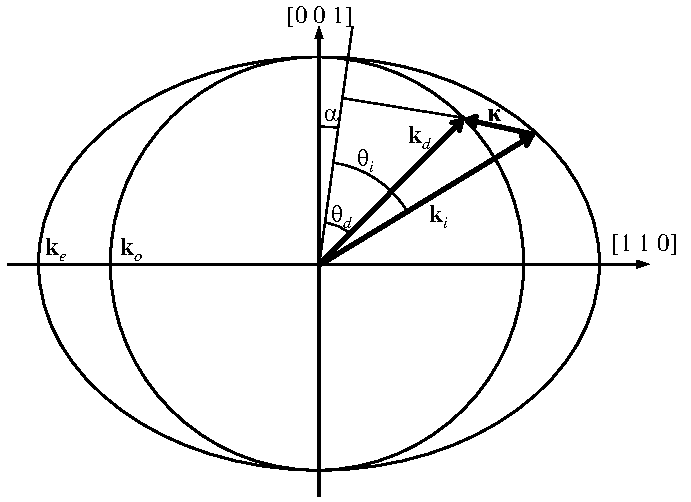
\includegraphics[width=120mm]{amt-2015-329-discussions-f01.pdf}
\caption{The wave vectors generated by the AOTF experiment. From
  Eq.~(1), the incident wave vector, $\vec{k}_{\mathrm{i}}$,
  diffracted wave vector, $\vec{k}_{\mathrm{d}}$, and acoustic wave
  vector $\boldsymbol{\kappa}$ are shown. The respective interaction
  angles for the incident and diffracted wave vectors
  $\theta_{\mathrm{i}}$ and $\theta_{\mathrm{d}}$ are also presented.}
\label{amtd-2015-0329-f01.pdf}
\end{figure}

\begin{figure}
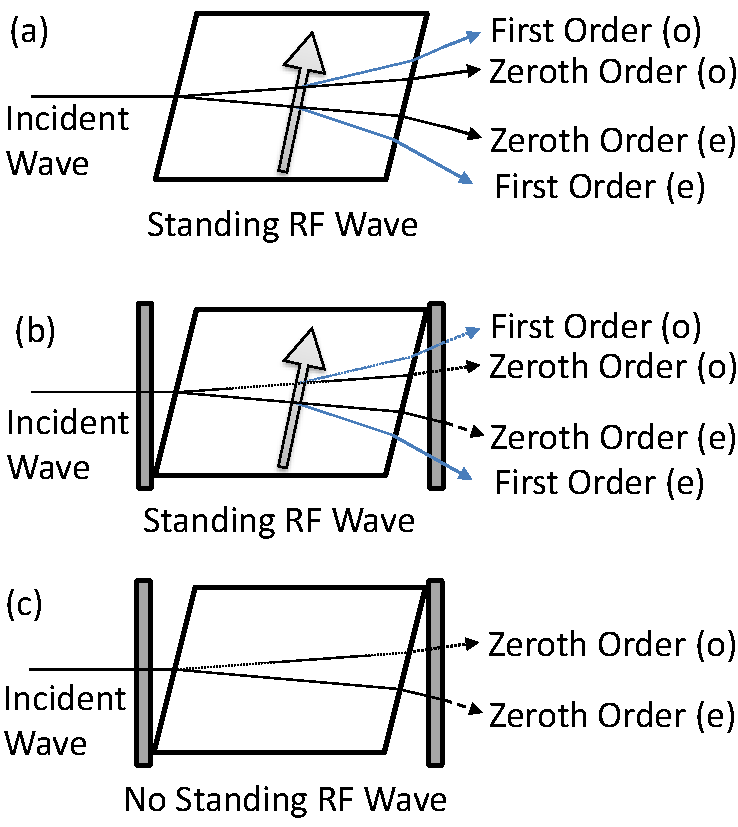
\includegraphics[height=90mm]{amt-2015-329-discussions-f02.pdf}
\caption{\textbf{(a)} A representative AOTF undergoing Bragg diffraction with an
  unpolarised incident wave with a~RF wave applied represented by the
  arrow. After the diffraction event four output signals are formed:
  the zeroth order and first order ordinary (o) and extraordinary (e)
  signals. However the only optical path that remains at a~constant
  angle no matter the applied RF wavelength is the first order
  extraordinary diffracted signal. \textbf{(b)} Two linear polarizers
  are added to the system, the first linear polarizer removes the
  ordinary polarization removing the outputs with the dotted lines and
  the second linear polarizer removes undiffracted extraordinary light
  shown by the dashed line. \textbf{(c)} The system in \textbf{(b)}
  without a~RF wave so Bragg diffraction is occurring. Once again the
  first linear polarizer removes the ordinary polarization represented
  by the dotted line and the second linear polarizer removes the
  extraordinary light shown by the dashed line.}
\label{amtd-2015-0329-f02.pdf}
\end{figure}

\begin{figure}
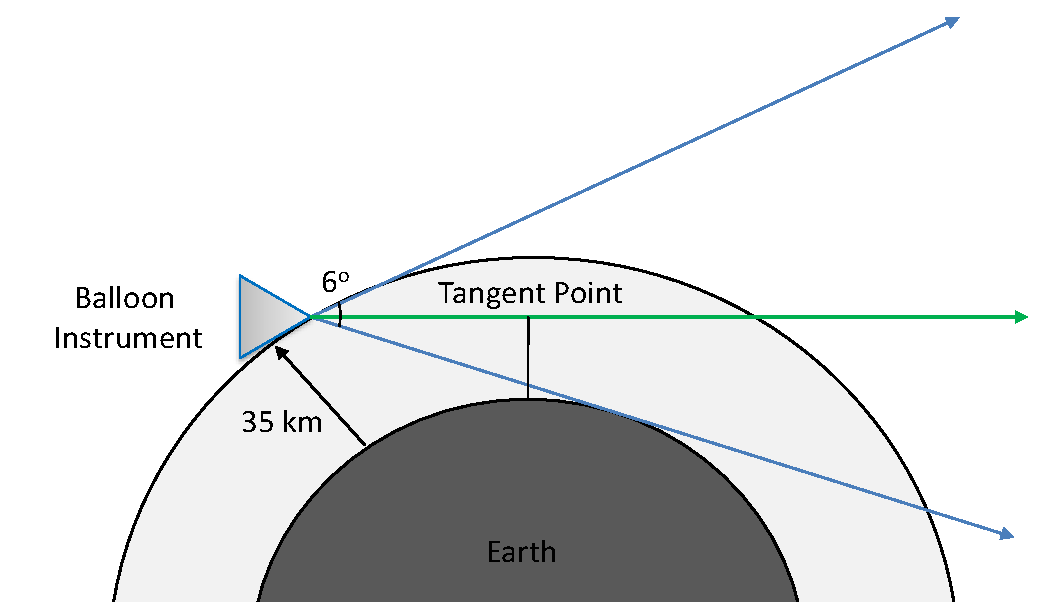
\includegraphics[width=120mm]{amt-2015-329-discussions-f03.pdf}
\caption{ALI in a~stratospheric balloon geometry showing the complete
  6{\degree} field of view in blue with a~float altitude of
  35\,\unit{km}. The green line shows a~typical vertical line-of-sight
  where the tangent point or altitude is set by the minimum distance
  between the earth and the line--of--sight.}
\label{amtd-2015-0329-f03.pdf}
\end{figure}

\begin{figure}
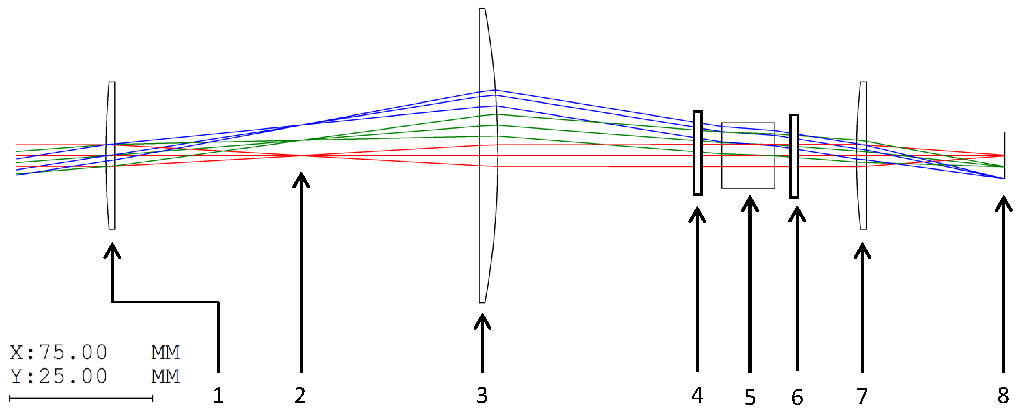
\includegraphics[width=120mm]{amt-2015-329-discussions-f04.pdf}
\caption{Ray Tracing diagram of the telescopic lens system for ALI
  simulated by Code V optical design software. The elements in the
  system are the following: (1) 150\,\unit{mm} focal length
  plano-convex lens. (2) Field stop.  (3) 100\,\unit{mm} focal length
  plano-convex lens. (4) Vertical linear polarizer.  (5) Brimrose
  AOTF. (6) Horizontal linear polarizer. (7) 50.4\,\unit{mm} focal
  length bi-convex lens. (8) Imaging plane.}
\label{amtd-2015-0329-f04.pdf}
\end{figure}

\begin{figure}
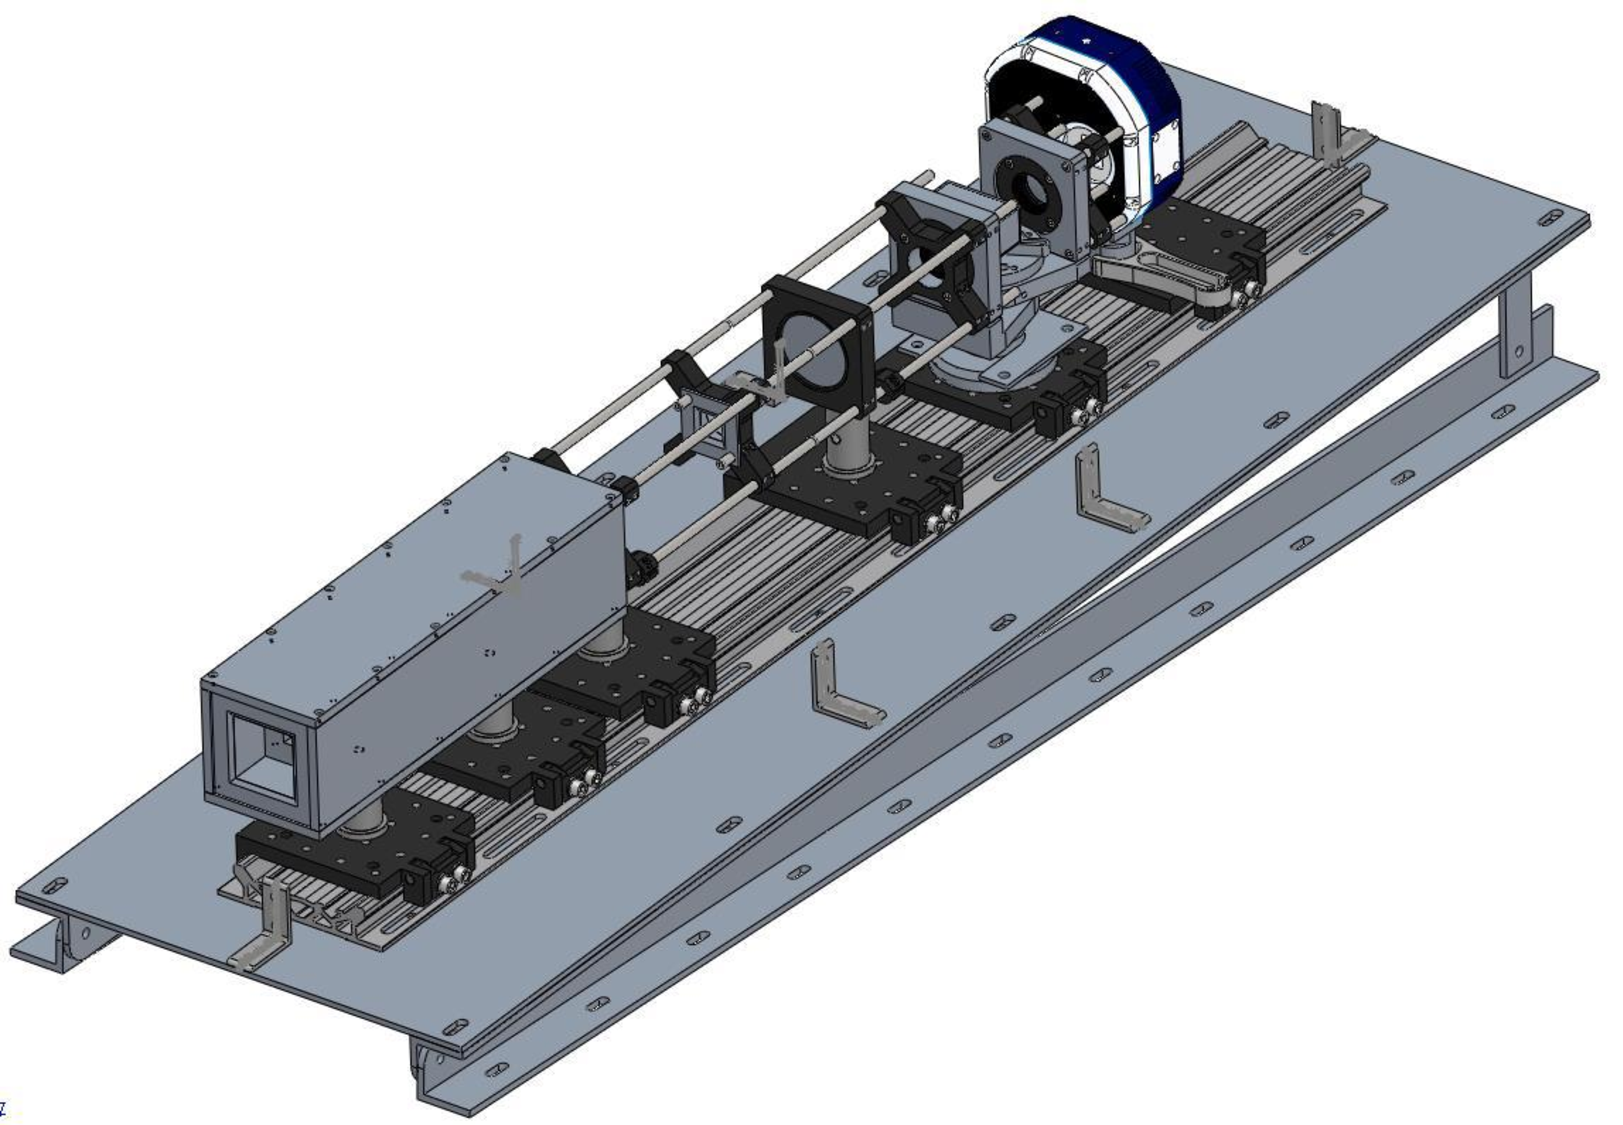
\includegraphics[width=120mm]{amt-2015-329-discussions-f05.pdf}
\caption{An isometric view of the complete ALI system with the baffle
  and 3{\degree} slant required to correctly position the field of
  view. Light tight case absent from diagram.}
\label{amtd-2015-0329-f05.pdf}
\end{figure}

\begin{figure}
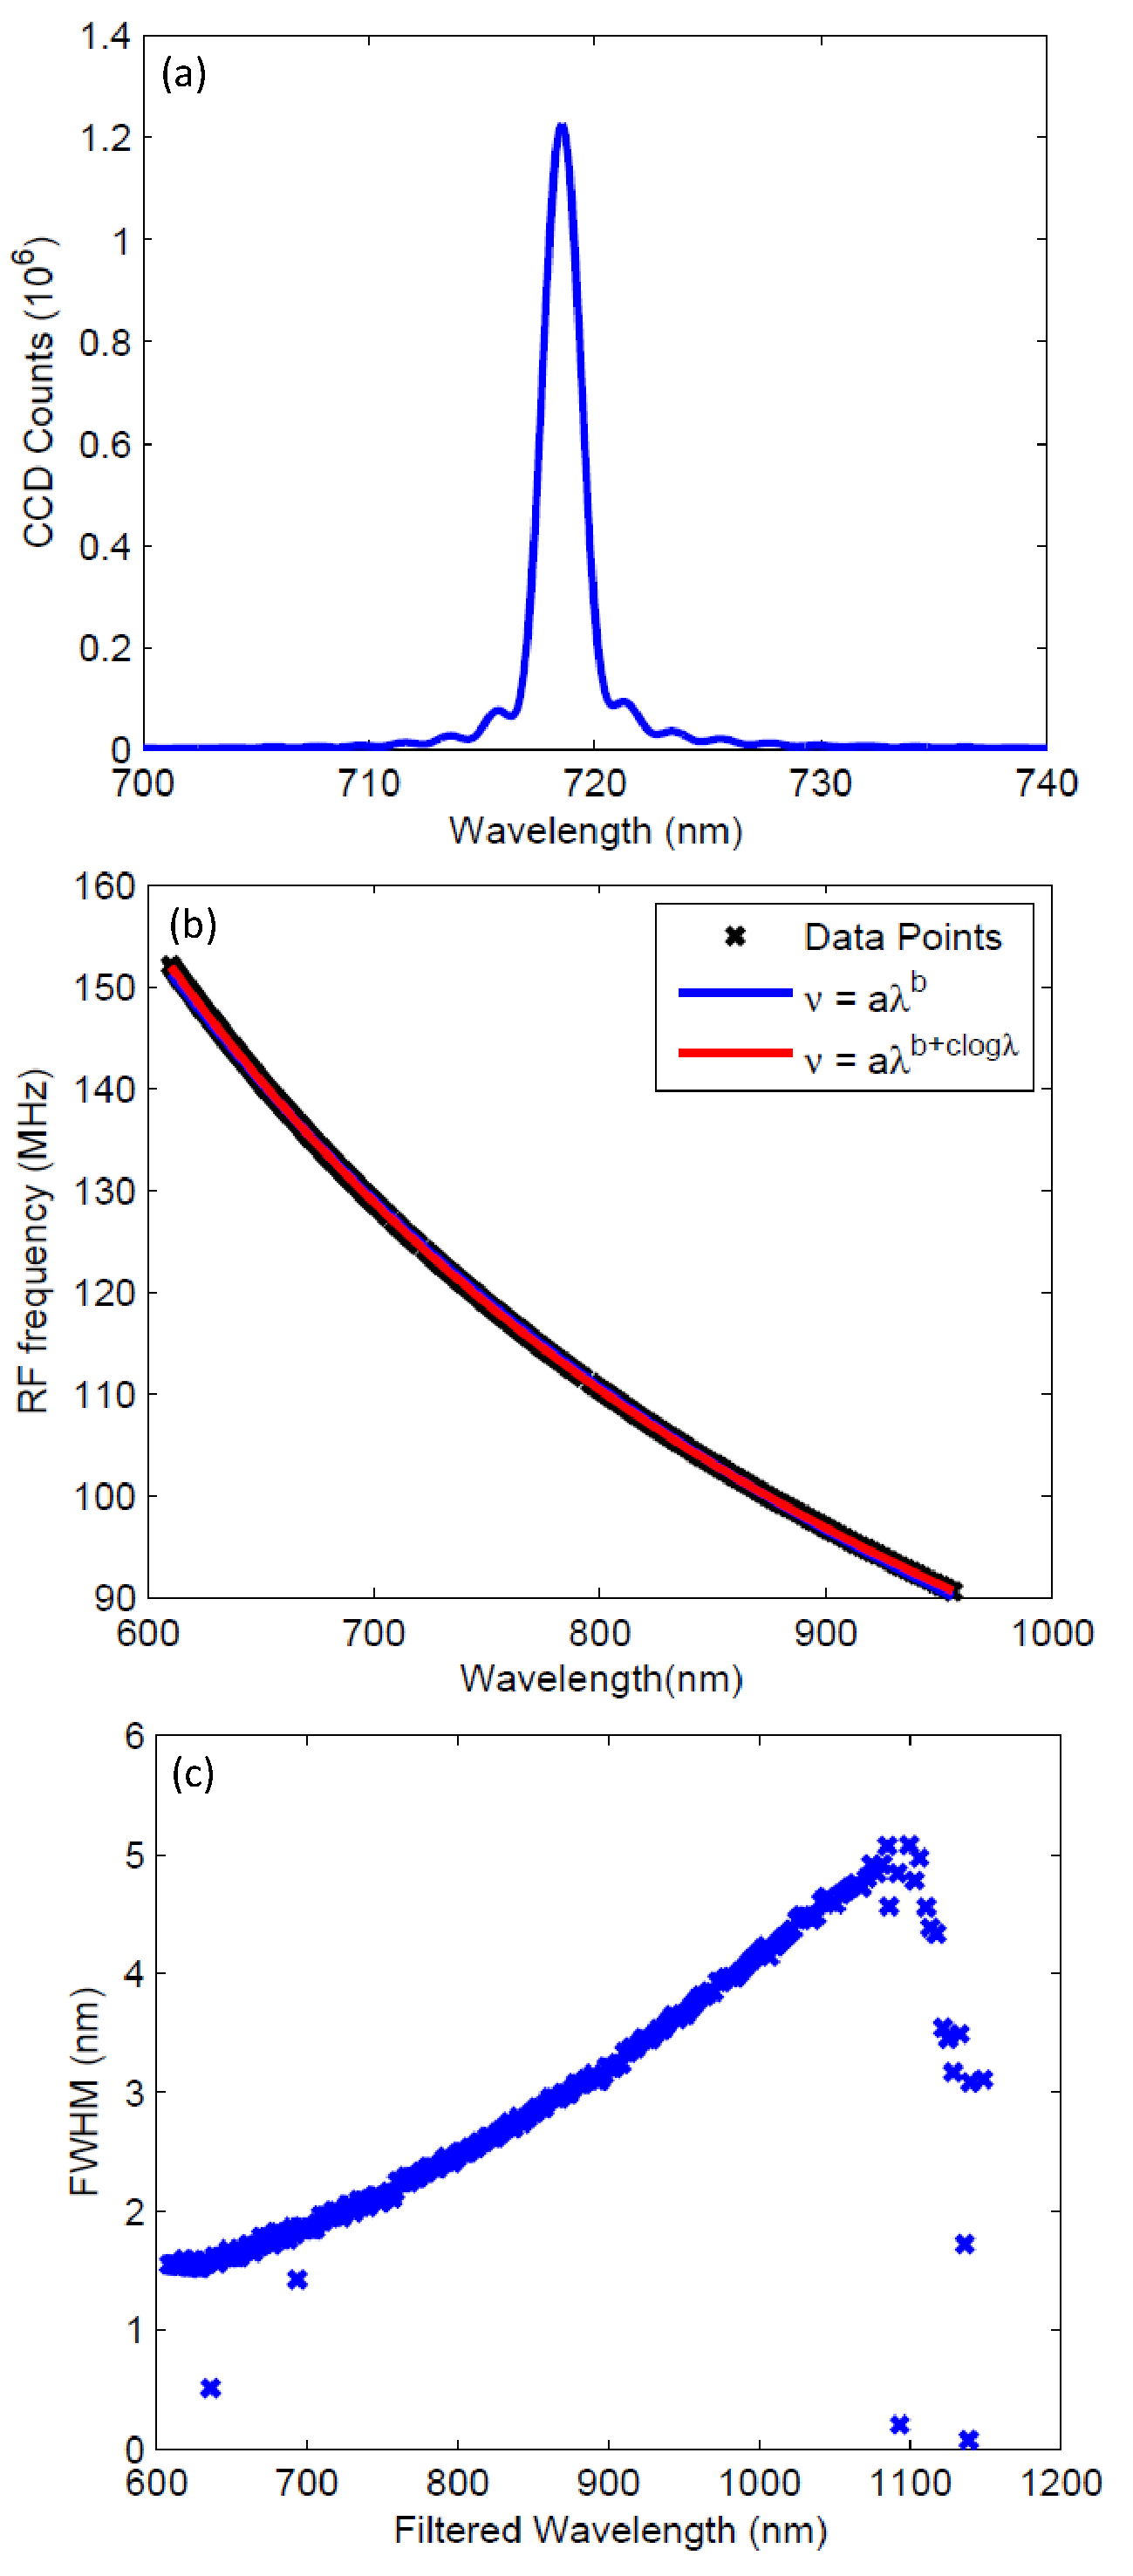
\includegraphics[height=110mm]{amt-2015-329-discussions-f06.pdf}
\caption{\textbf{(a)} A~spectrum taken from the AOTF from the point
  spread function when the tuning frequency of the AOTF was at
  124.96\,\unit{MHz}. \textbf{(b)} The calibration curves for the AOTF
  tuning curve which contains the data points recorded and fit
  curve. \textbf{(c)} The full width half max for each of the
  determined wavelengths for the AOTF. The full width half max at
  600\,\unit{nm} is 1.5\,\unit{nm} and as the wavelengths get longer
  it increases to 4.9\,\unit{nm} at 1080\,\unit{nm}.}
\label{amtd-2015-0329-f06.pdf}
\end{figure}

\begin{figure}
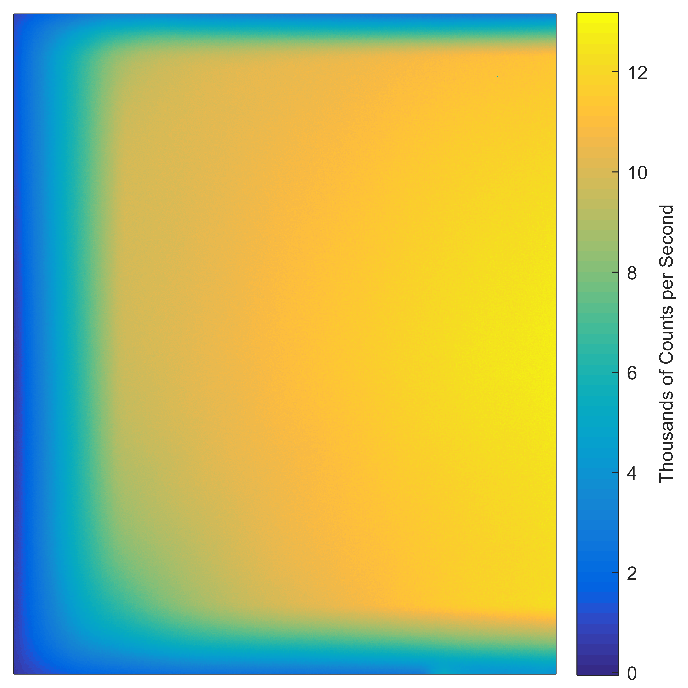
\includegraphics[height=110mm]{amt-2015-329-discussions-f07.pdf}
\caption{A~calibration image after stray light removal has been
  performed where the measured wavelength is 750\,\unit{nm} with
  a~1\,s exposure time.  Vignetting can be seen as moving away from
  center of the image. Additionally the last 1{\degree} of the
  horizontal field of view on the right side is lost due to strong
  contamination from reflections within the system.}
\label{amtd-2015-0329-f07.pdf}
\end{figure}

\begin{figure}
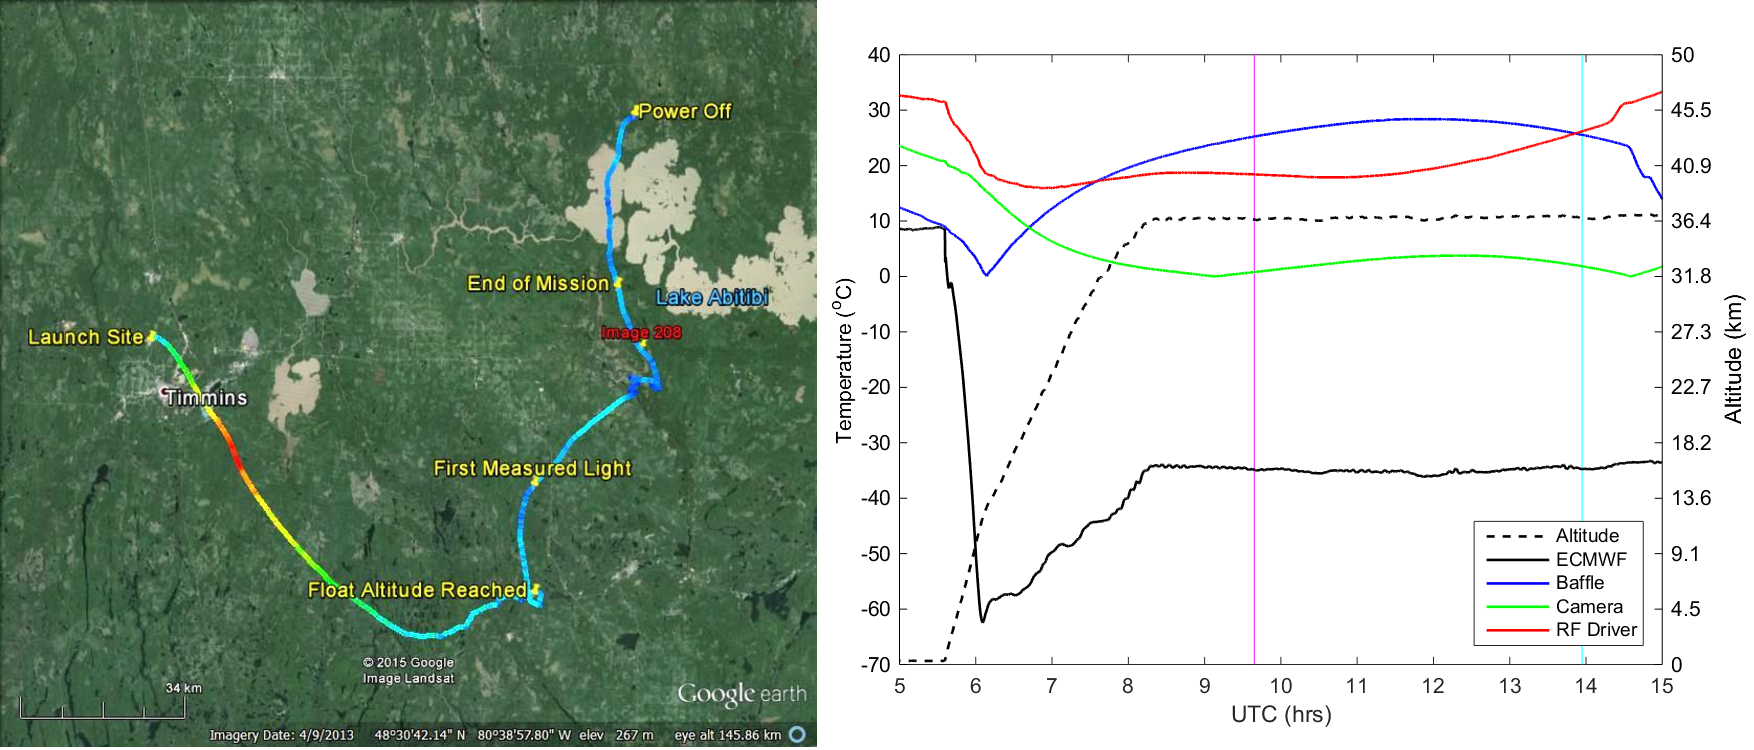
\includegraphics[width=120mm]{amt-2015-329-discussions-f08.pdf}
\caption{\textbf{(a)} The GPS data from ALI during the Nimbus 7
  mission generated via Google Earth. The colour of the line
  represents the absolute speed of the gondola during the
  mission and the blue, green, red colours represent speeds of approximately
  10, 70, and 140~km/h. Important landmarks are noted on the image.  The end of
  mission represent the end of the aerosol mission. No GPS data was
  collected from ALI after power down. The location of image 208 is
  the red label. \textbf{(b)} The temperature and altitude profiles
  from the NIMBUS 7 flight.  The time of image 208 is shown by the
  cyan vertical line and first light measured by ALI is represented by the
  magenta vertical line.}
\label{amtd-2015-0329-f08.pdf}
\end{figure}

\begin{figure}
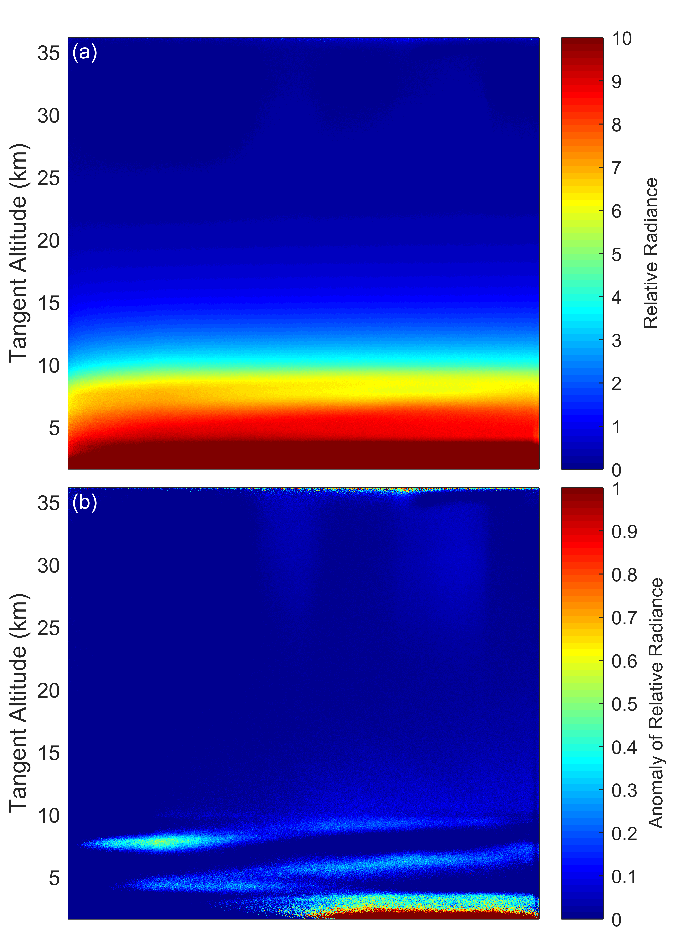
\includegraphics[height=110mm]{amt-2015-329-discussions-f09.pdf}
\caption{\textbf{(a)} Final calibrated 750\,\unit{nm} image, taken at
  13:57\,UTC located at 48.55{\degree}\,N, 80.00{\degree}\,W with
  a~solar zenith angle and solar scattering angle of 63 and
  98{\degree} respectively. \textbf{(b)} The same 750\,\unit{nm} image
  with the mean of the profile removed from the image leaving the
  residual signal that shows thin clouds in the troposphere.}
\label{amtd-2015-0329-f09.pdf}
\end{figure}

\begin{figure}
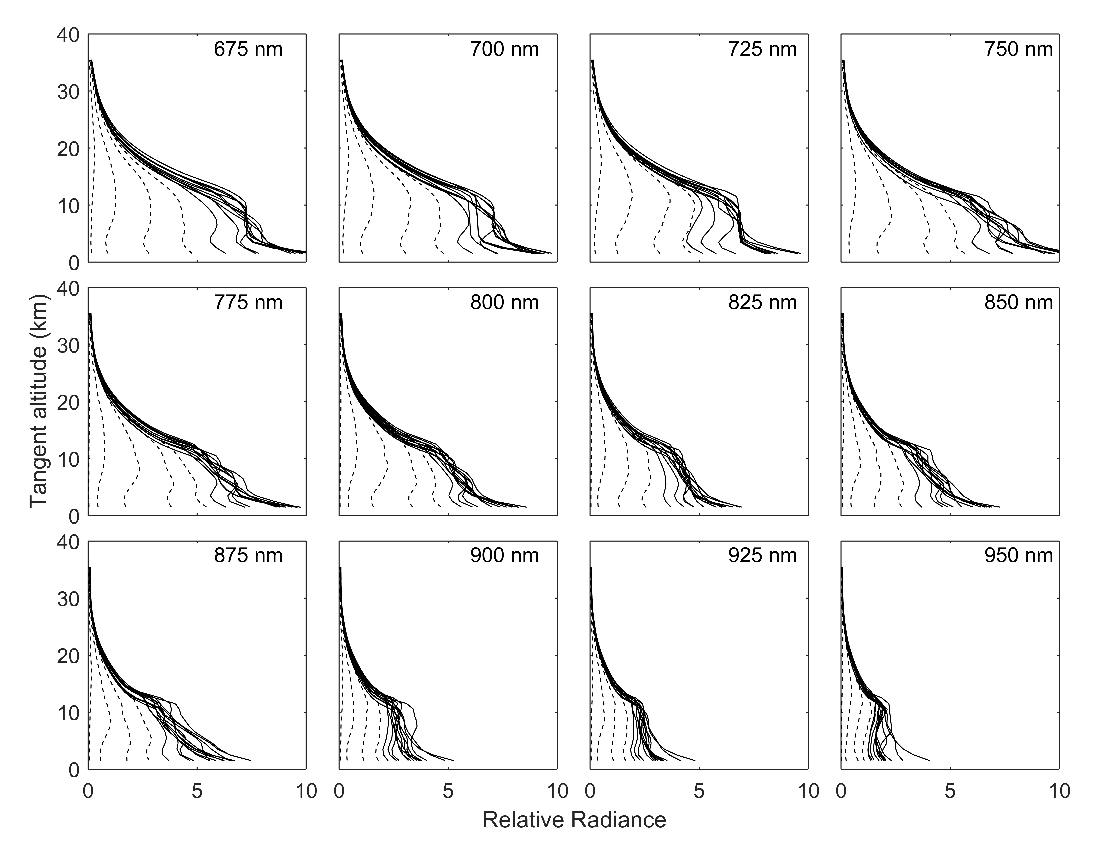
\includegraphics[width=120mm]{amt-2015-329-discussions-f10.pdf}
\caption{Averaged ALI relative radiance vectors from 12 of the 13
  wavelengths from the NIMBUS-7 flight. Each panel presents the
  radiance vectors from a~different wavelength measured which is
  denoted in the top right corner. The dashed lines are radiance
  profiles where the solar zenith angle is greater than 90{\degree}
  and solid lines are profile where the solar zenith angle is less
  than 90{\degree}. The separation between each consecutive radiance vector at each wavelength is approximately 2 degrees in solar zenith angle. }
\label{amtd-2015-0329-f10.pdf}
\end{figure}

\begin{figure}
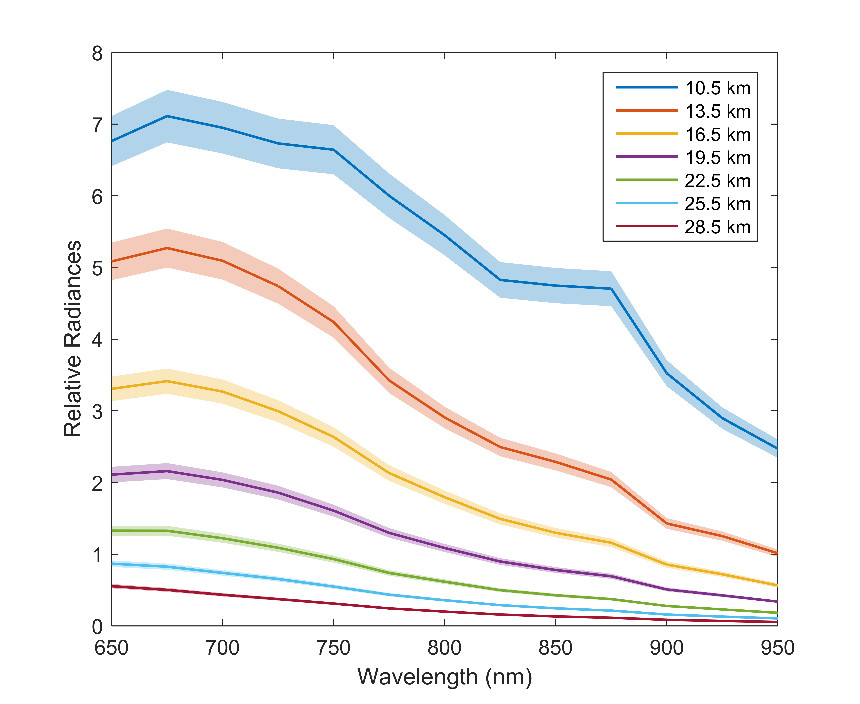
\includegraphics[width=120mm]{amt-2015-329-discussions-f11.pdf}
\caption{Level 1 relative radiances spectrally from 650 to
  950\,\unit{nm} as measured from ALI at approximately 14:20\,UTC
  consisting of images number 204 to 216 looking 90{\degree} in the
  azimuth from the sun facing southwards. These spectral profiles are
  presented at several tangent altitudes with a~horizontal look
  direction of 0{\degree}. The shading represents the error on the
  radiances.}
\label{amtd-2015-0329-f11.pdf}
\end{figure}

\begin{figure}
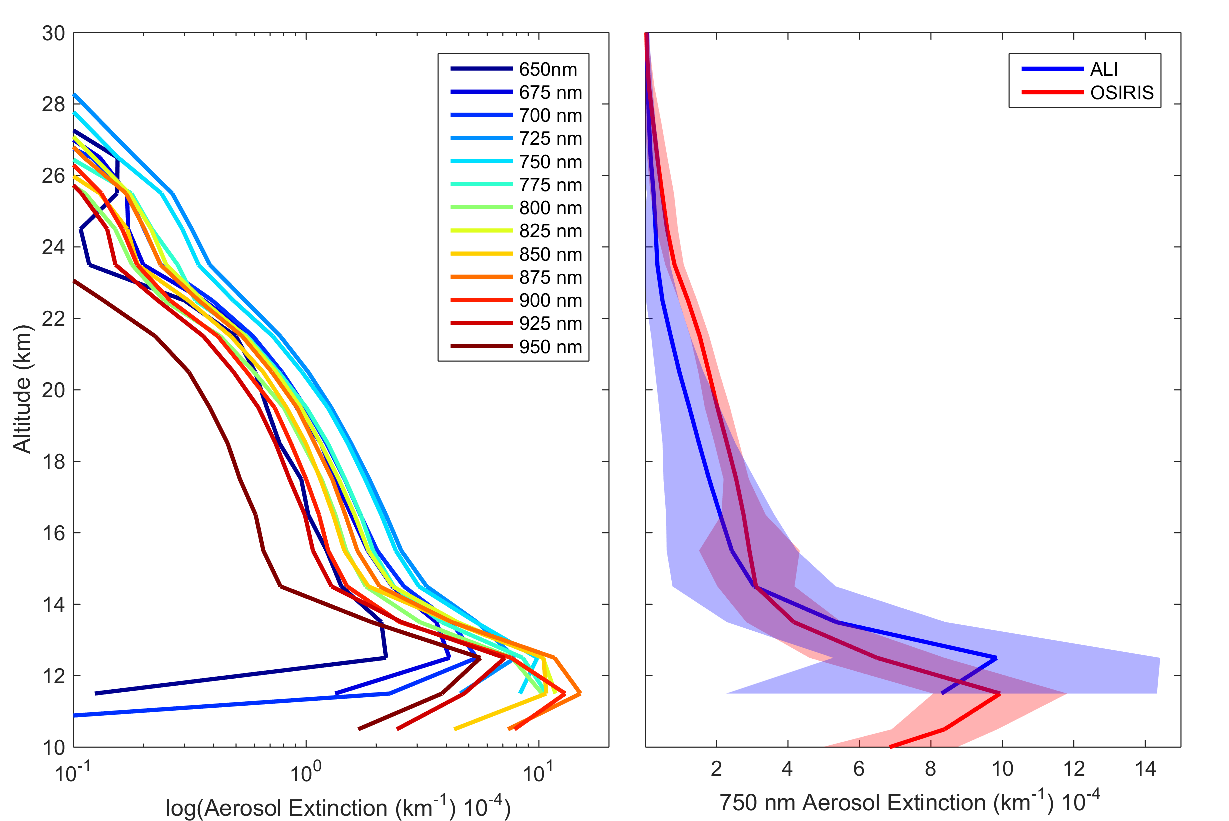
\includegraphics[width=120mm]{amt-2015-329-discussions-f12.pdf}
\caption{Left is the retrieved aerosol extinction profiles from the
  last complete imaging cycle consisting of images 205 to 216 from the
  0.0{\degree} horizontal line-of-sight. Right is the 750\,\unit{nm}
  ALI aerosol extinction in blue compared to the 750\,\unit{nm} extinction measured by OSIRIS
  in red with its error represented by the respective
  shading.}
\label{amtd-2015-0329-f12.pdf}
\end{figure}

\begin{figure}
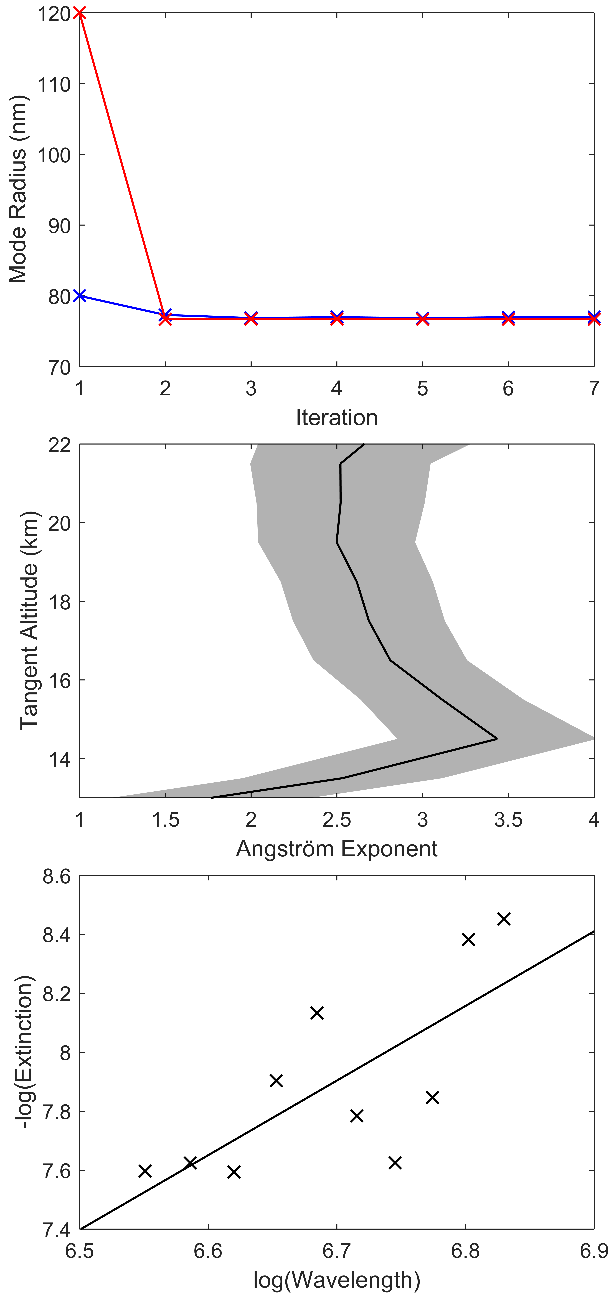
\includegraphics[height=100mm]{amt-2015-329-discussions-f13.pdf}
\caption{The top panel shows the convergence of two sample particle
  size retrievals, blue and red represent an initial state of 0.08 and
  0.12\,\unit{{\mu}m} mode radius respectively. Both initial states
  converge to the same value over approximately 3 iterations in the
  particle size retrieval method. The middle panel shows the final
  Angstr\"{o}m exponents determined from images 204--216. The shading
  represents the error associated with the least squares fit. The
  bottom panel shows a~typical least squares fit of the retrieved
  extinction values over wavelength to determine the Angstr\"{o}m
  exponent at model altitude of 14.5\,\unit{km}.}
\label{amtd-2015-0329-f13.pdf}
\end{figure}

\end{document}

\endinput
